\documentclass[conference]{IEEEtran}

% para correr / compilar 
% pdflatex main.tex
% bibtex main
% pdflatex main.tex
% pdflatex main.tex
% 

\usepackage[spanish]{babel}
\usepackage{amsmath,amssymb,amsfonts,amsthm}
\usepackage[utf8]{inputenc} % Caracteres en Español (Acentos, ñs)
\usepackage{csquotes}
\usepackage{graphicx}
\usepackage{url} % ACENTOS
\usepackage{hyperref} % Referencias
\usepackage{subfig}
\usepackage{lipsum}
\usepackage{balance} 
\usepackage{etoolbox}
\usepackage{datetime}
\usepackage{float}
\makeatletter
\patchcmd{\frontmatter@RRAP@format}{(}{}{}{}
\patchcmd{\frontmatter@RRAP@format}{)}{}{}{}
\makeatother	

\usepackage[backend=bibtex,sorting=none]{biblatex}
\setcounter{biburllcpenalty}{7000}
\setcounter{biburlucpenalty}{8000}
\addbibresource{references.bib}

% fecha
\usepackage{datetime}
\newdateformat{specialdate}{
    \twodigit{\THEDAY}-\twodigit{\THEMONTH}-\THEYEAR
}
\date{\specialdate\today}

% la sentencia \burl en las citas... 
\usepackage[hyphenbreaks]{breakurl}
\renewcommand\spanishtablename{Tabla}
\renewcommand\spanishfigurename{Figura}


\begin{document}
% Definitions
\newcommand{\breite}{0.9} %  for twocolumn
\newcommand{\RelacionFiguradoscolumnas}{0.9}
\newcommand{\RelacionFiguradoscolumnasPuntoCinco}{0.45}

%Title of paper
\title{Proyecto en Equipo U1 \\ Detección de Piedras en los Frijoles}

% Trabajo Individual
\author{
    \IEEEauthorblockN{
        Ricardo Emmanuel Uriegas Ibarra\IEEEauthorrefmark{1}
    }
    \IEEEauthorblockN{
        Hector Israel Cruz Resendez\IEEEauthorrefmark{1}
    }
    \IEEEauthorblockN{
        Dael Tovar Escamilla\IEEEauthorrefmark{1}
    }
    \IEEEauthorblockN{
        Jose Angel Alfaro Zurita\IEEEauthorrefmark{1}
    }
    % En caso de trabajos en equipo, poner a todos los autores 
    % en estricto ORDEN ALFABETICO
    %\author{\IEEEauthorblockN{Michael Shell\IEEEauthorrefmark{1},
    %Homer Simpson\IEEEauthorrefmark{1}}
    \IEEEauthorblockA{
        \IEEEauthorrefmark{1}Ingeniería en Tecnologías de la Información\\
        Universidad Politécnica de Victoria
    }
}

\maketitle

%%%%%%%%%%%%%%%%%%%%%%%%%%%%%%%%%%%%%%%%%%%%%%%%%%%%%%%%%%%%%%%%%%%%%%%
\begin{abstract} 
    En este documento se describe un sistema para detectar piedras en frijoles solamente mediante procesamiento de imágenes. Utilizando separación de color, operaciones morfológicas y análisis de contornos, se identifican piedras en frijoles pintos y negros. El sistema aplica umbrales (HSV o LAB), usa OpenCV para la segmentación y cuya interfaz es desarrollada usando PyQt6. Aunque logra resultados consistentes bajo condiciones controladas, si considerásemos un entorno completamente variable, la robustez del sistema podría verse comprometida.
\end{abstract}

%%%%%%%%%%%%%%%%%%%%%%%%%%%%%%%%%%%%%%%%%%%%%%%%%%%%%%%%%%%%%%%%%%%%%%%
\section{Introducción}
    La detección de piedras en los frijoles es un problema común en la industria alimentaria, ya que la presencia de piedras en los frijoles puede dañar los molinos y causar problemas de salud en los consumidores. En este trabajo se propone un sistema para la detección de piedras en los frijoles, utilizando solamente análisis de imágenes. El sistema se basa en la identificación de diferencias morfológicas y de color entre los frijoles y las piedras, sin recurrir a redes neuronales. 
    
    El sistema se propone como una alternativa a los métodos ya existentes en la detección de piedras en los frijoles\cite{limpieza}.

%%%%%%%%%%%%%%%%%%%%%%%%%%%%%%%%%%%%%%%%%%%%%%%%%%%%%%%%%%%%%%%%%%%%%%%
\section{Desarrollo Experimental}
    En este trabajo se desarrollo un sistema capaz de detectar piedras en los frijoles dada una foto (sin usar ningún tipo de red neuronal). Para ello se utiliza la librería OpenCV\cite{opencv} en Python\cite{python}, en combinación de la librería PyQt6\cite{pyqt6} para la interfaz gráfica.
    Debido a las limitaciones de tiempo y recursos, se desarrolla el sistema solamente para 2 tipos de frijoles; pinto y negro. 

    \subsection{Características del Frijol}
    \subsubsection{Frijol Pinto}
    El frijol pinto tiene las siguientes características:
    \begin{enumerate}
        \item Frijol color cafe claro con manchas cafe oscuro.
        \item Las piedras que llegan a aparecer en este tipo de frijoles son color negro.
        \item Forma ovalada.
        \item Textura lisa.
    \end{enumerate}

    \subsubsection{Frijol Negro}
    El frijol negro tiene las siguientes características:
    \begin{enumerate}
        \item Color negro uniforme con un punto blanco en el hilum\cite{semillas}.
        \item Las piedras que llegan a aparecer en este tipo de frijoles son color gris claro (cercano al color hueso\cite{pantone}).
        \item Forma ovalada.
        \item Textura lisa.
    \end{enumerate}

    \subsection{Características de las Fotos}
    Para el desarrollo del proyecto es necesario conseguir un conjunto de pruebas que permitan verificar su correcto funcionamiento. Este conjunto de pruebas son fotos tomadas con un celular \textit{iPhone SE 2020}\cite{iphone} con dimesiones de $4,032 \times 3,024$ o $3,024 \times 4,032$, esto debido a que era el celular disponible por uno de los participantes del proyecto.

    Las imagen se tomaron con flash (tratando de evitar sombras que puedan interferir con el análisis de la imagen) y llevaran un fondo blanco o equivalente, mientras los frijoles se encontraran esparcidos a lo largo de la imagen, sin algun patron aparente.

    \subsection{Procesamiento previo al Análisis de la Imagen}
    Se realizan los siguientes pasos para preprocesar la imagen:
    \begin{itemize}
        \item La imagen se carga y se redimensiona para ajustarse al tamaño de la interfaz gráfica.
        \item Se crea una copia en formato OpenCV para realizar el procesamiento.
        \item Para frijoles negros, se reduce la imagen (escala 0.5) y se convierte a espacio HSV, permitiendo aplicar máscaras basadas en umbrales específicos y operaciones morfológicas (estos valores se obtuvieron a prueba y error) para eliminar ruido.
        \item Para frijoles pintos, la imagen se transforma al espacio LAB y se aplican umbrales en sus canales, junto a filtros morfológicos (de igual manera también se obtuvieron a prueba y error), para resaltar las piedras.
        \item Se utiliza el color dominante de la imagen para elegir la vía de procesamiento adecuada.
    \end{itemize}
    
    \subsection{Segmentación de las Piedras}
    Con base en el preprocesamiento, la segmentación se realiza de la siguiente forma:
    \begin{enumerate}
        \item Se aplica una máscara para cada color: en HSV para frijoles negros y en LAB para frijoles pintos (esto porque al estar realizando la detección de frijoles pintos se leyó\cite{lab} que LAB era superior a HSV)
        \item Se emplean operaciones morfológicas para reducir pequeños ruidos y cerrar huecos en la imagen afectada por la máscara\ref{fig:mascara_negros}\ref{fig:mascara_pintos}.
        \item Se extraen los contornos utilizando la función \textit{findContours} de OpenCV.
        \item Los contornos se filtran en función de criterios calculados a prueba y error:
        \begin{itemize}
            \item Para frijoles negros, se consideran aquellos con área entre 1350 y 8000 píxeles, ratio de convexidad superior a 0.5 y al menos 5 vértices.
            \item Para frijoles pintos, se filtran con área mayor a 1200 píxeles, circularidad entre 0.15 y 0.65, ratio de convexidad mayor a 0.4 y entre 6 y 15 vértices.
        \end{itemize}
        \item Finalmente, se resaltan dichos contornos sobre la imagen original para visualizar la detección de piedras.
    \end{enumerate}

    El color de las piedras se obtuvo utilizando la herramienta \textit{ColorPicker}\cite{colorpicker} que viene integrada en el entorno de escritorio KDE con el paquete \textit{kdeplasma-addons}. Cada tipo de frijol se maneja de forma diferente debido a la diferencia de entornos de las fotos.

    \subsection{Interfaz Gráfica}
    La interfaz gráfica se desarrollo en PyQt6\cite{pyqt6} y consta de 2 secciones principales:
    \begin{enumerate}
        \item Sección de carga de imagen: Donde se carga la imagen a analizar.
        \item Sección de resultados: Donde se muestra la imagen original con los objetos detectados de manera destacada.
    \end{enumerate}

%%%%%%%%%%%%%%%%%%%%%%%%%%%%%%%%%%%%%%%%%%%%%%%%%%%%%%%%%%%%%%%%%%%%%%%
\section{Resultados}
    En la figura \ref{fig:res1} se muestra la interfaz del sistema. Mientras tanto, la figura \ref{fig:res2} muestra un ejemplo de la detección de piedras en frijoles pintos. Por último, la figura \ref{fig:res3} muestra un ejemplo de la detección de piedras en frijoles negros.

    % images/UI.png
    \begin{figure}[H]
        \centering
        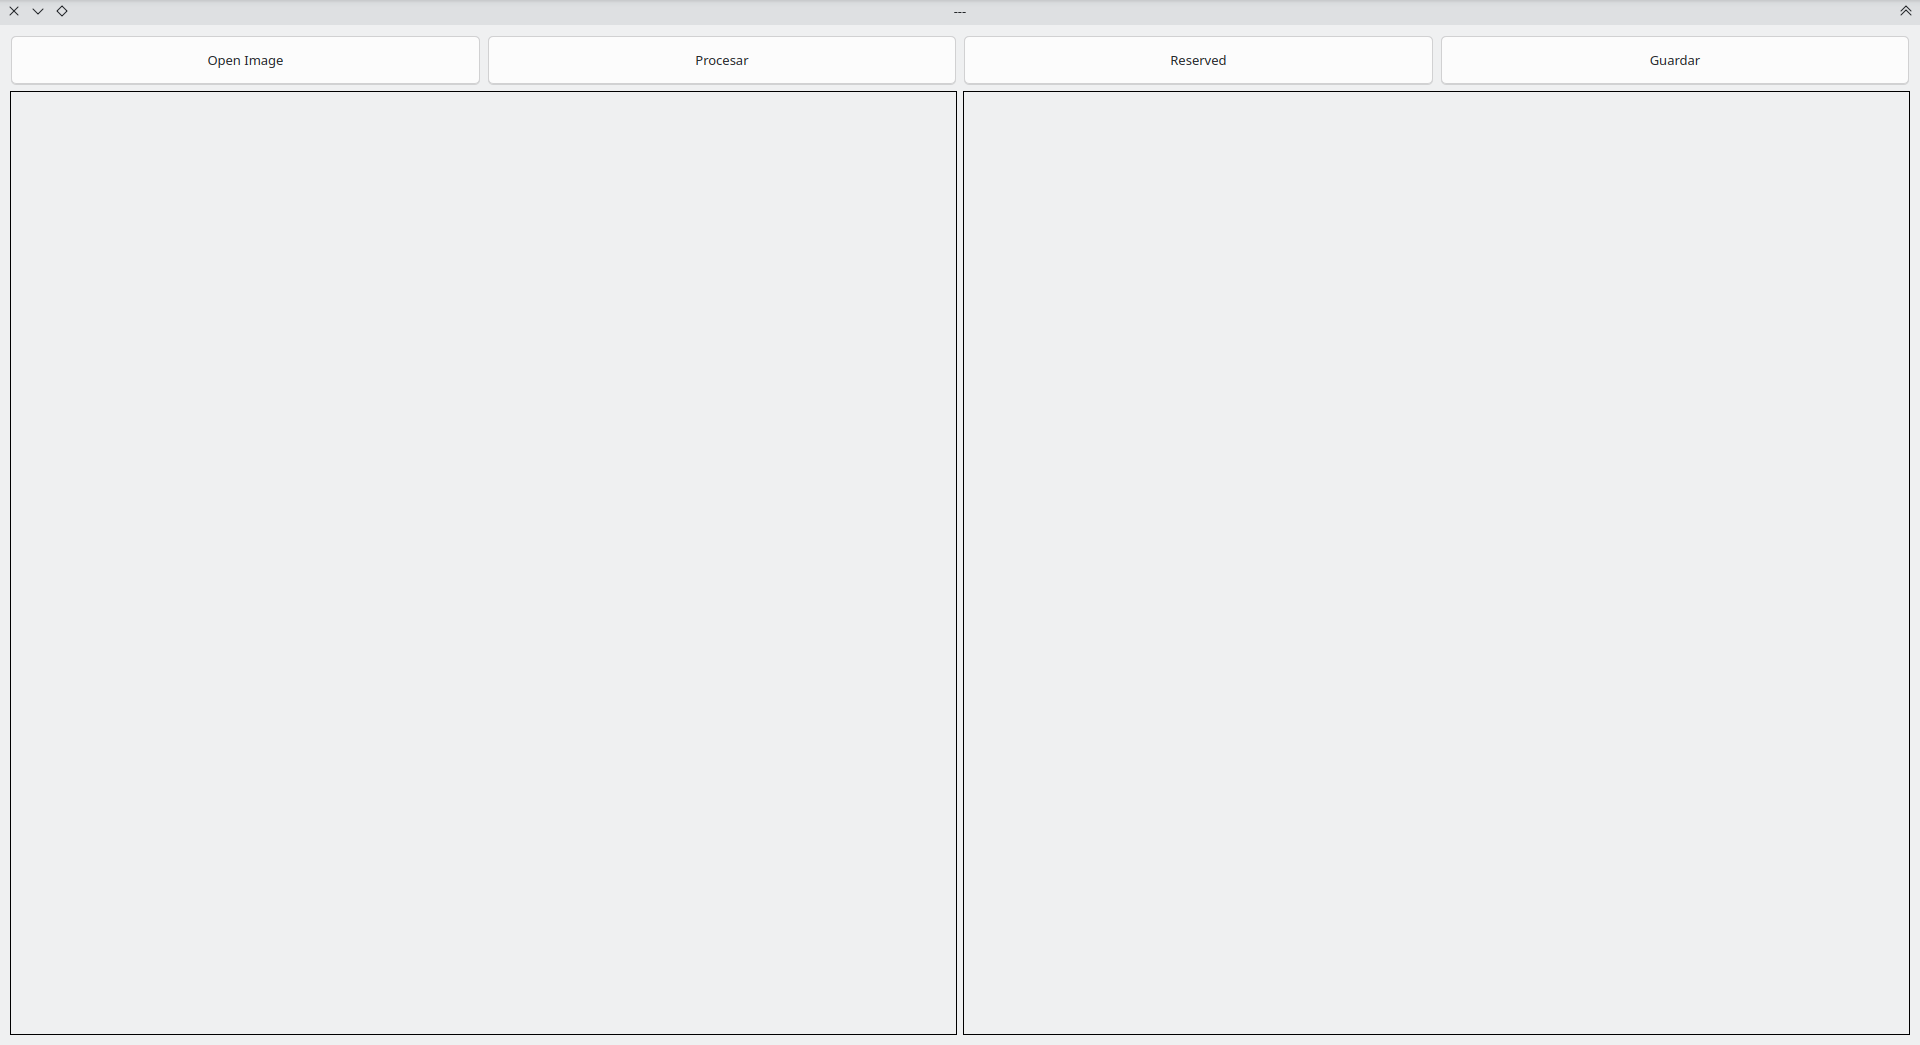
\includegraphics[width=\breite\linewidth]{images/UI.png}
        \caption{Interfaz del Sistema}
        \label{fig:res1}
    \end{figure}

    % images/pintos.png
    \begin{figure}[H]
        \centering
        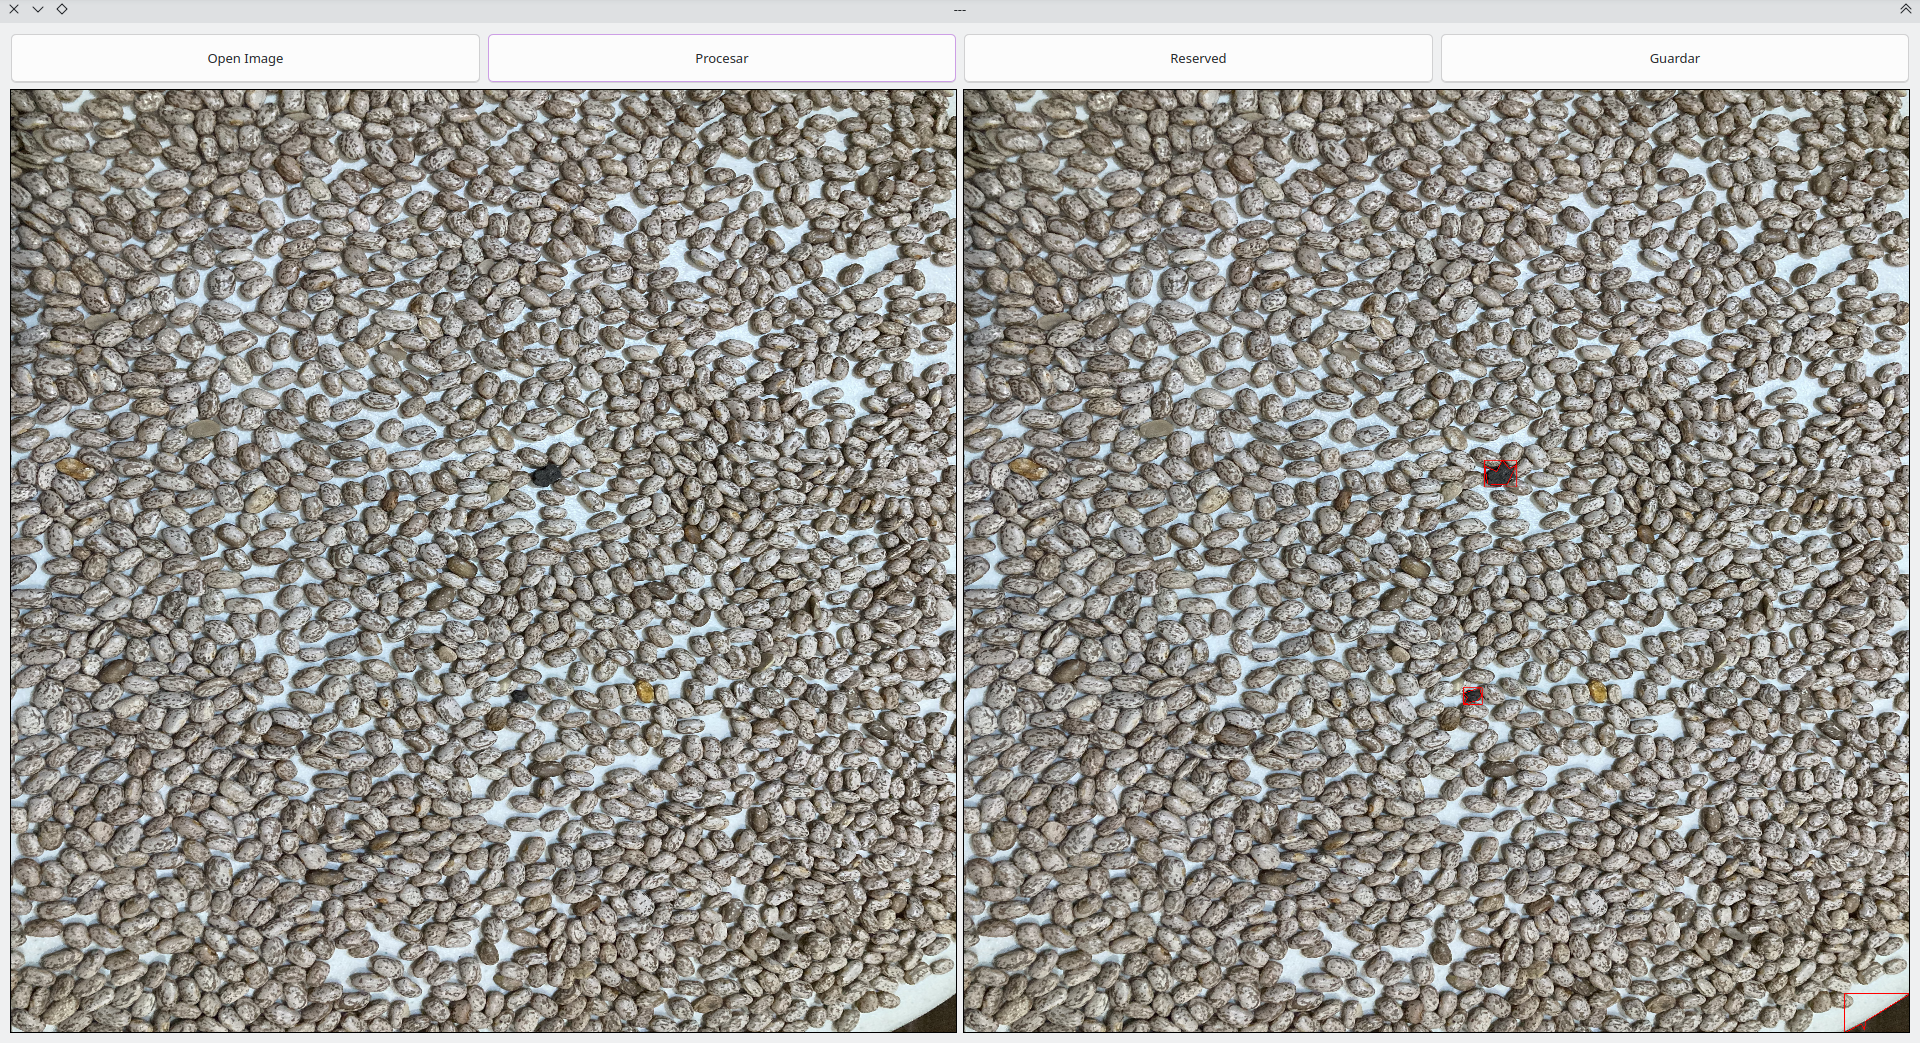
\includegraphics[width=\breite\linewidth]{images/pintos.png}
        \caption{Ejemplificación de la detección de piedras en los frijoles pintos}
        \label{fig:res2}
    \end{figure}

    % images/negros.png
    \begin{figure}[H]
        \centering
        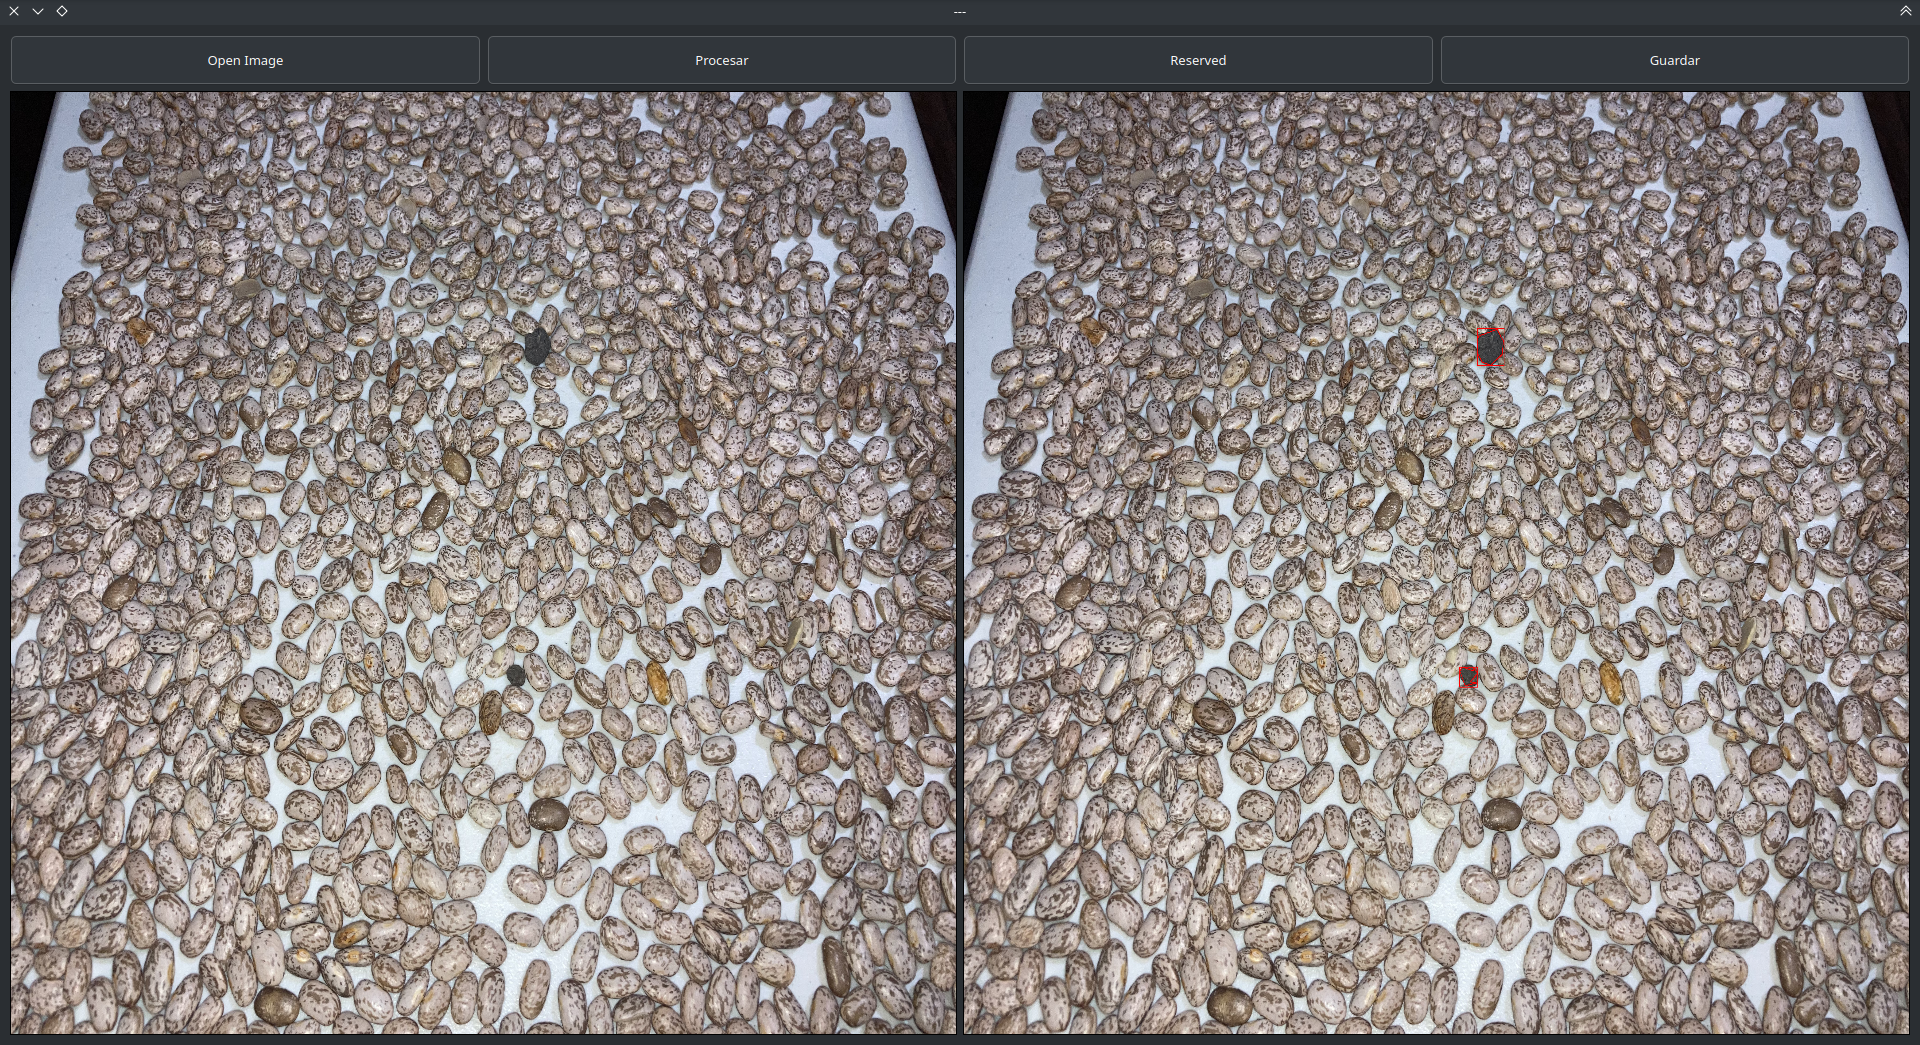
\includegraphics[width=\breite\linewidth]{images/negros.png}
        \caption{Ejemplificación de la detección de piedras en los frijoles negros}
        \label{fig:res3}
    \end{figure}

    Los casos que se muestran son exitosos. A continuación se muestran las pruebas con imágenes nada controladas que incluso llegan a incumplir una calidad de imagen parecida a las imágenes que se probaron al realizar el programa, lo cual demuestra la baja robustez del sistema desarrollado.

        % test1.png
        \begin{figure}[H]
            \centering
            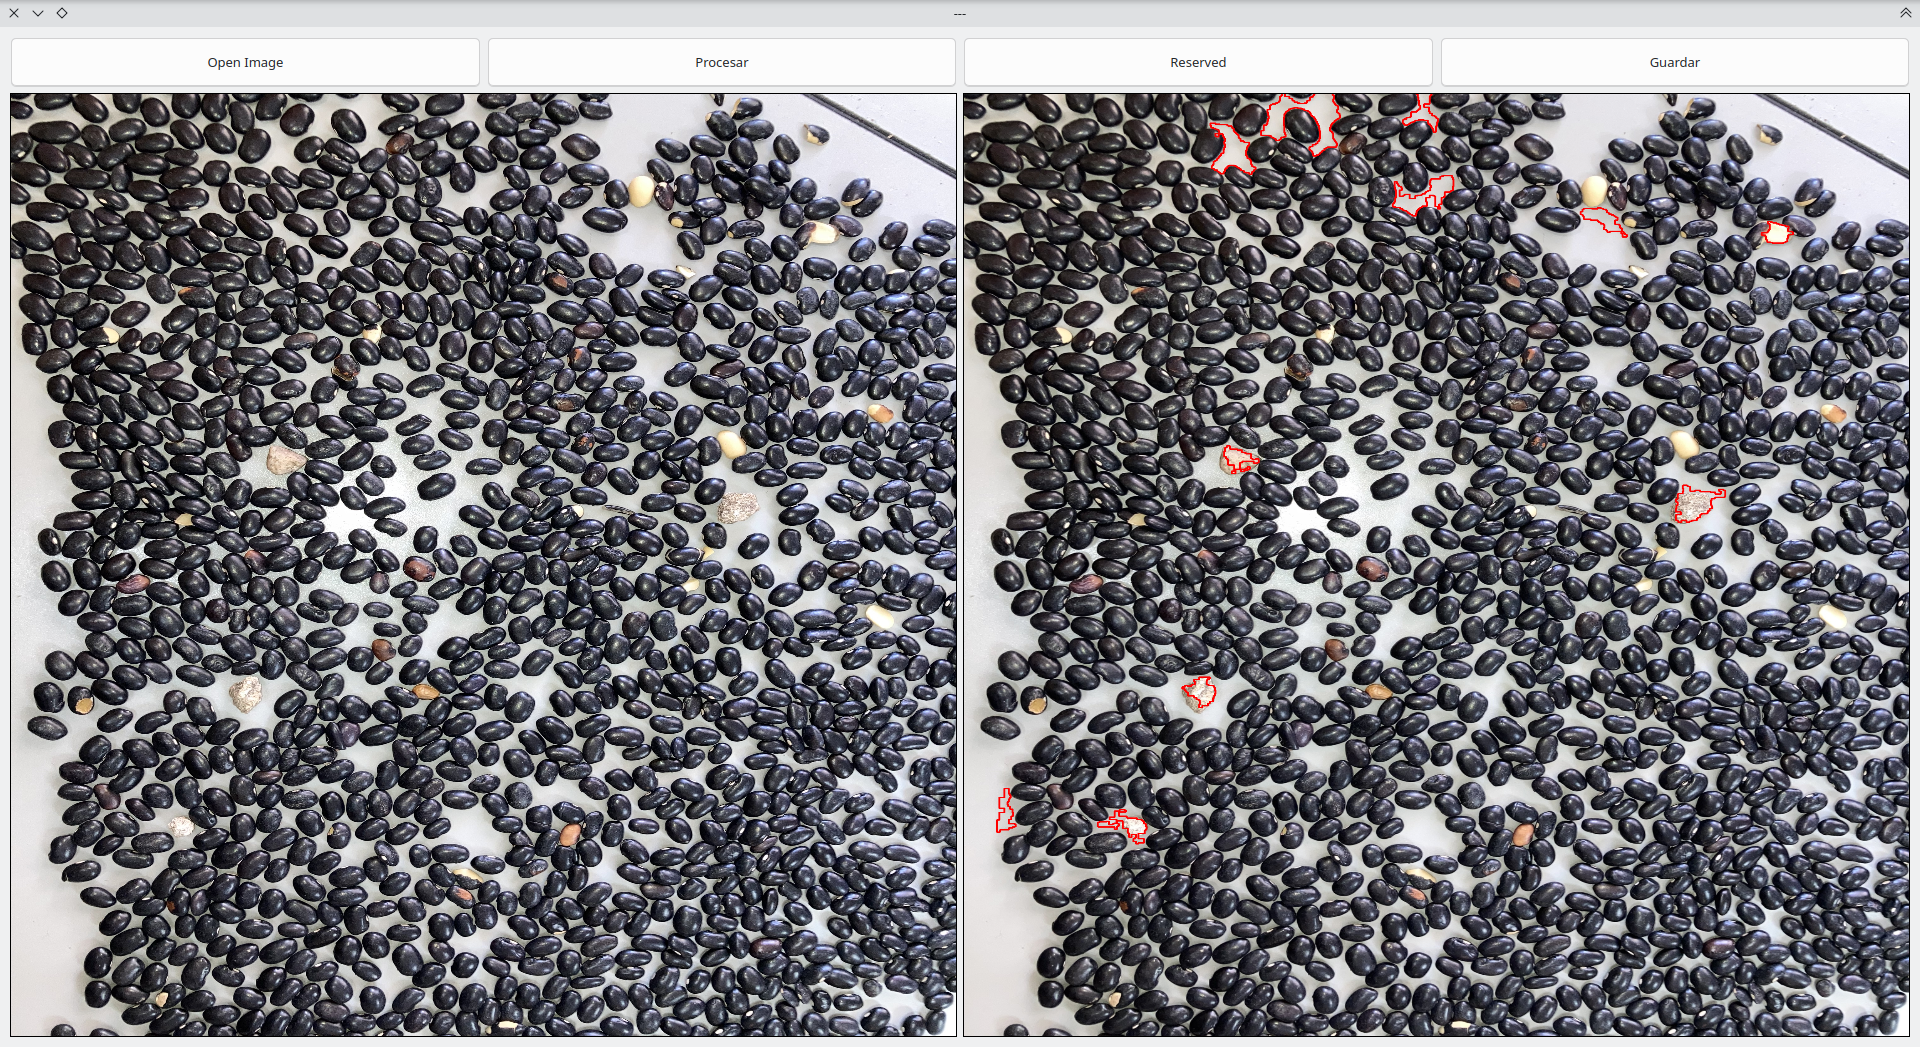
\includegraphics[width=\breite\linewidth]{images/test1.png}
            \caption{Resultados para test 1}
            \label{fig:test1}
        \end{figure}

        \begin{figure}[H]
            \centering
            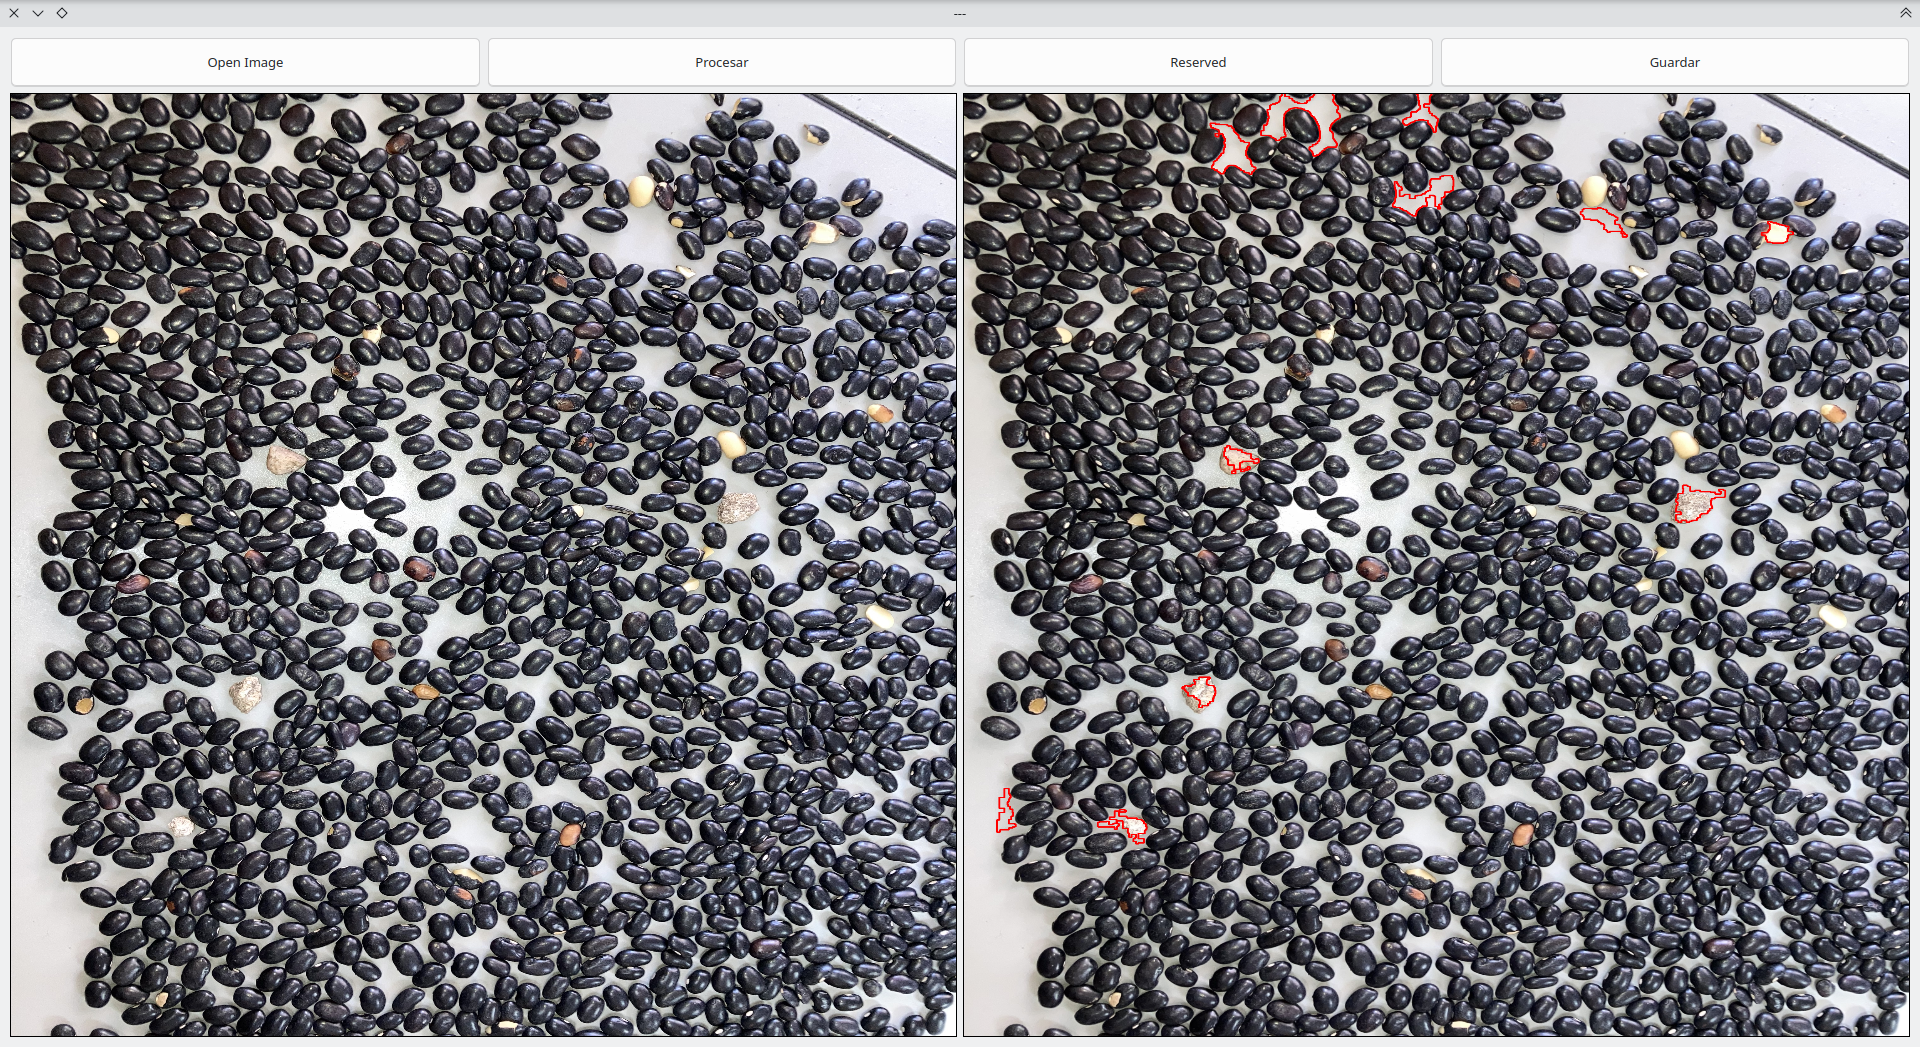
\includegraphics[width=\breite\linewidth]{images/test2.png}
            \caption{Resultados para test 2}
            \label{fig:test2}
        \end{figure}

        \begin{figure}[H]
            \centering
            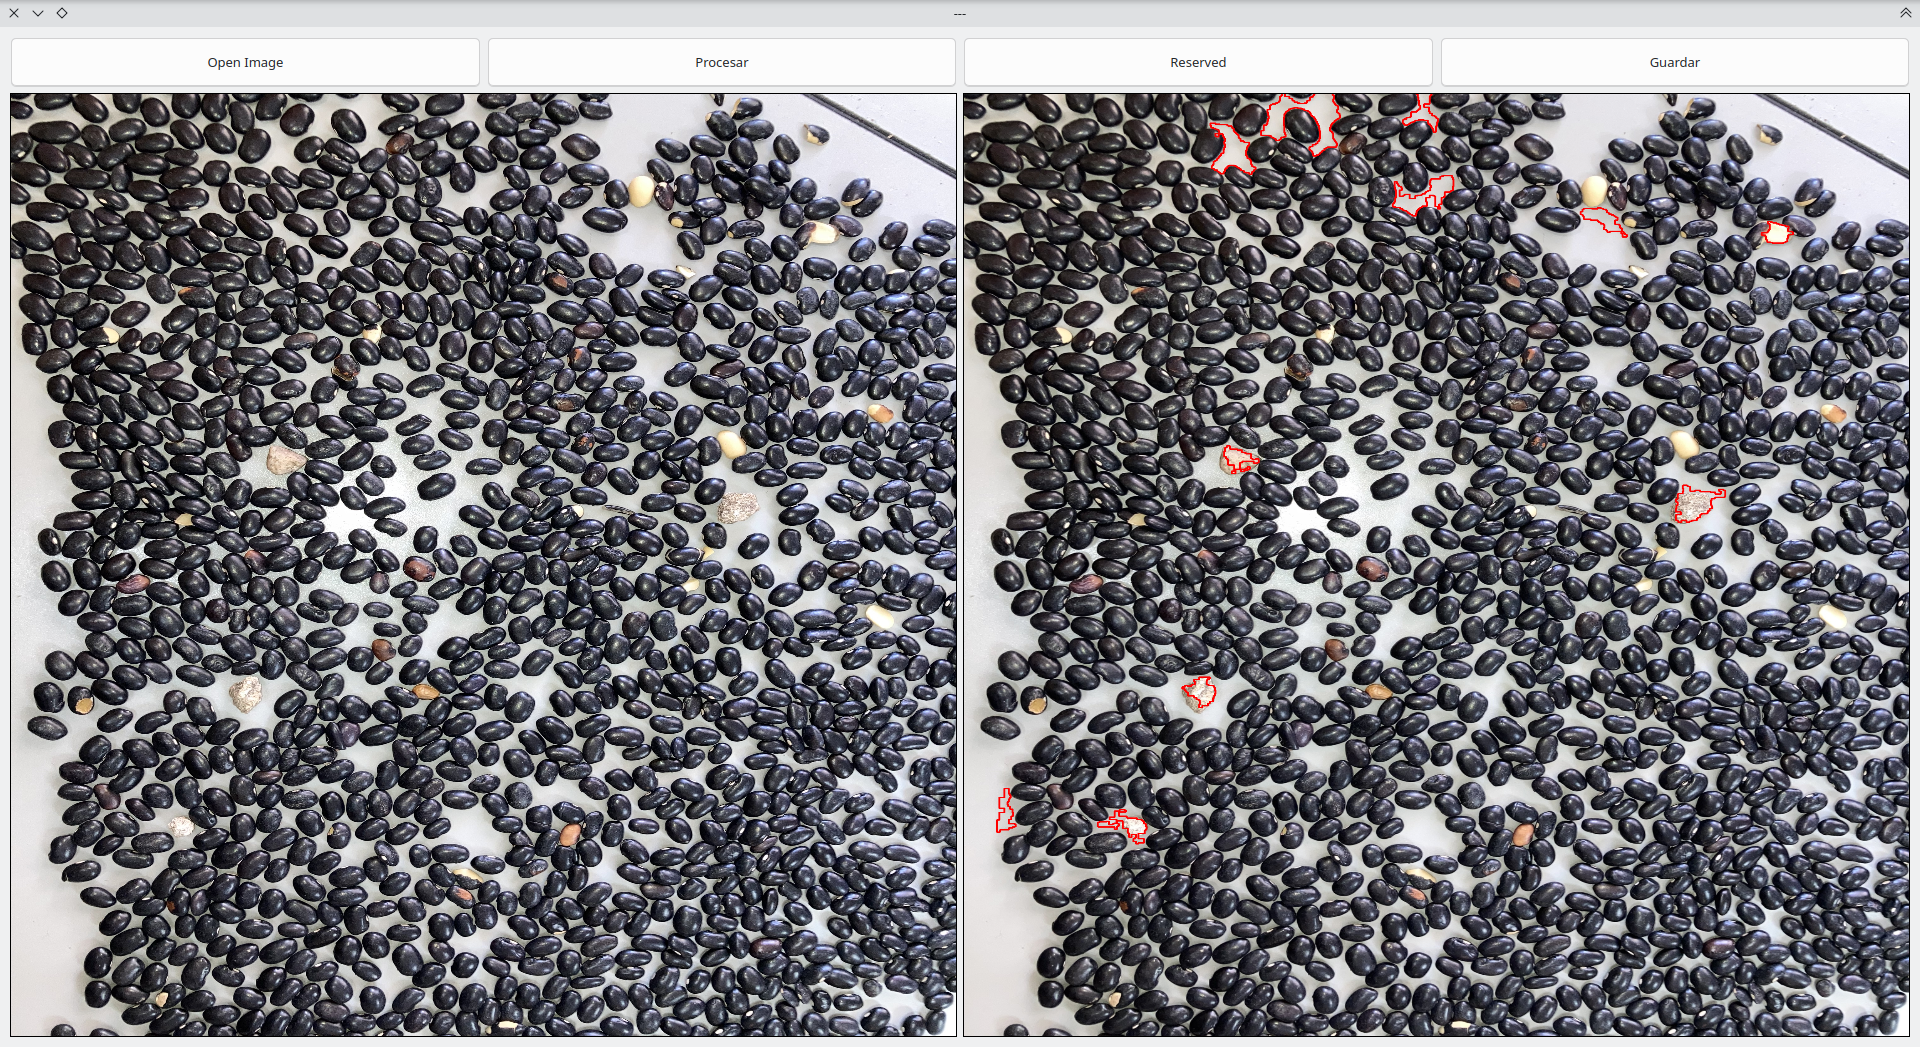
\includegraphics[width=\breite\linewidth]{images/test3.png}
            \caption{Resultados para test 3}
            \label{fig:test3}
        \end{figure}

        \begin{figure}[H]
            \centering
            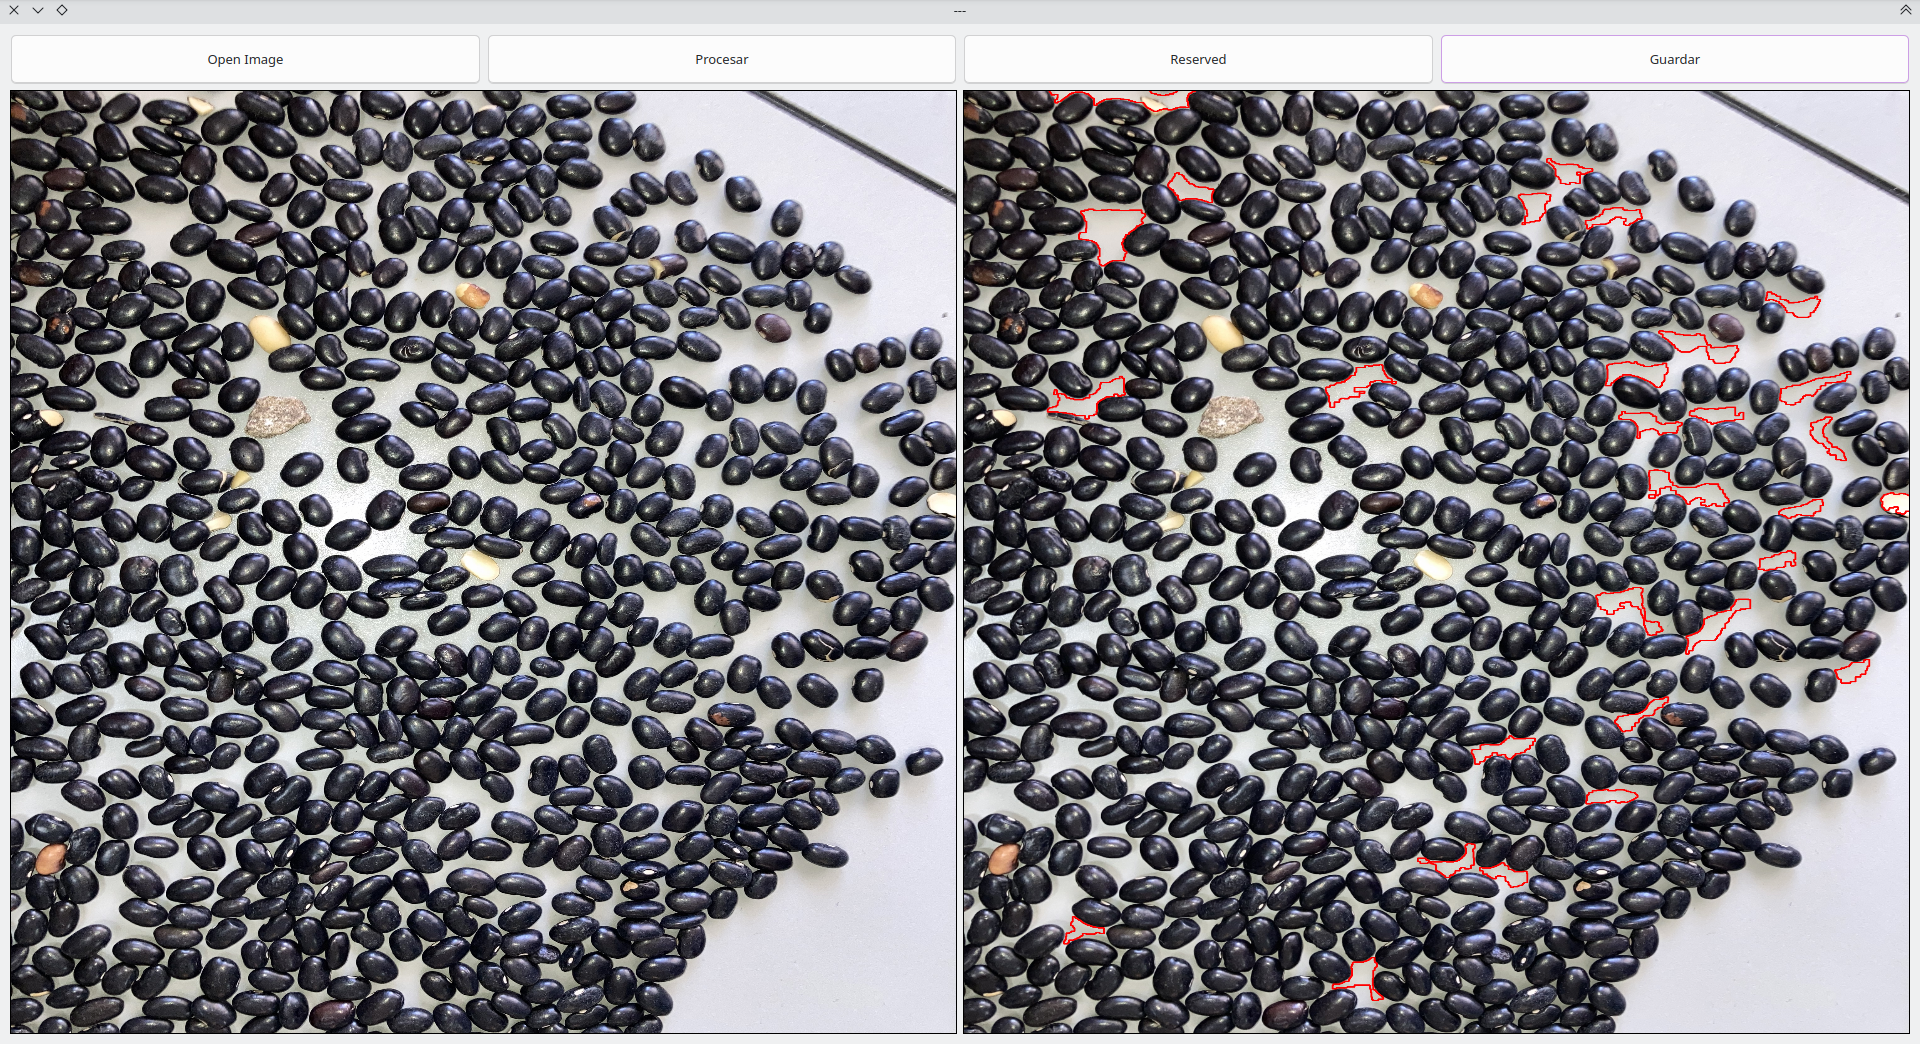
\includegraphics[width=\breite\linewidth]{images/test4.png}
            \caption{Resultados para test 4}
            \label{fig:test4}
        \end{figure}

        \begin{figure}[H]
            \centering
            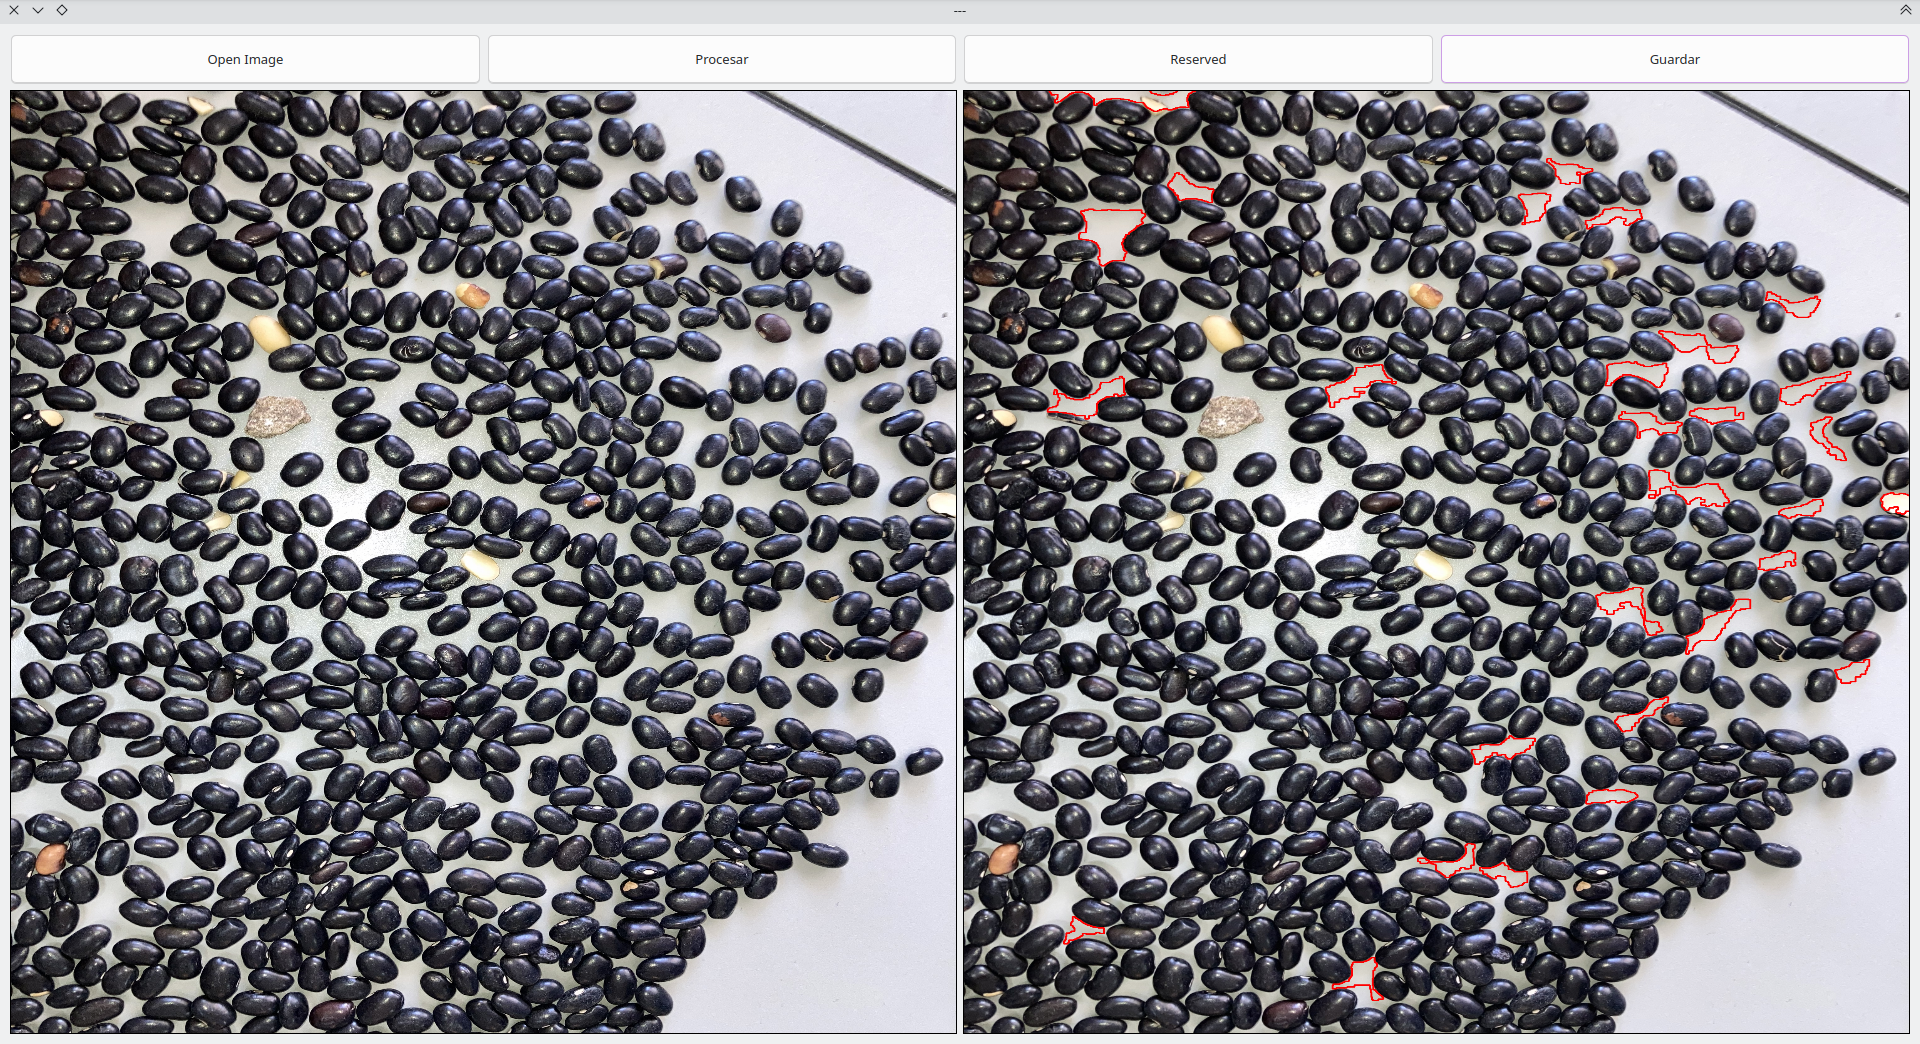
\includegraphics[width=\breite\linewidth]{images/test5.png}
            \caption{Resultados para test 5}
            \label{fig:test5}
        \end{figure}

        \begin{figure}[H]
            \centering
            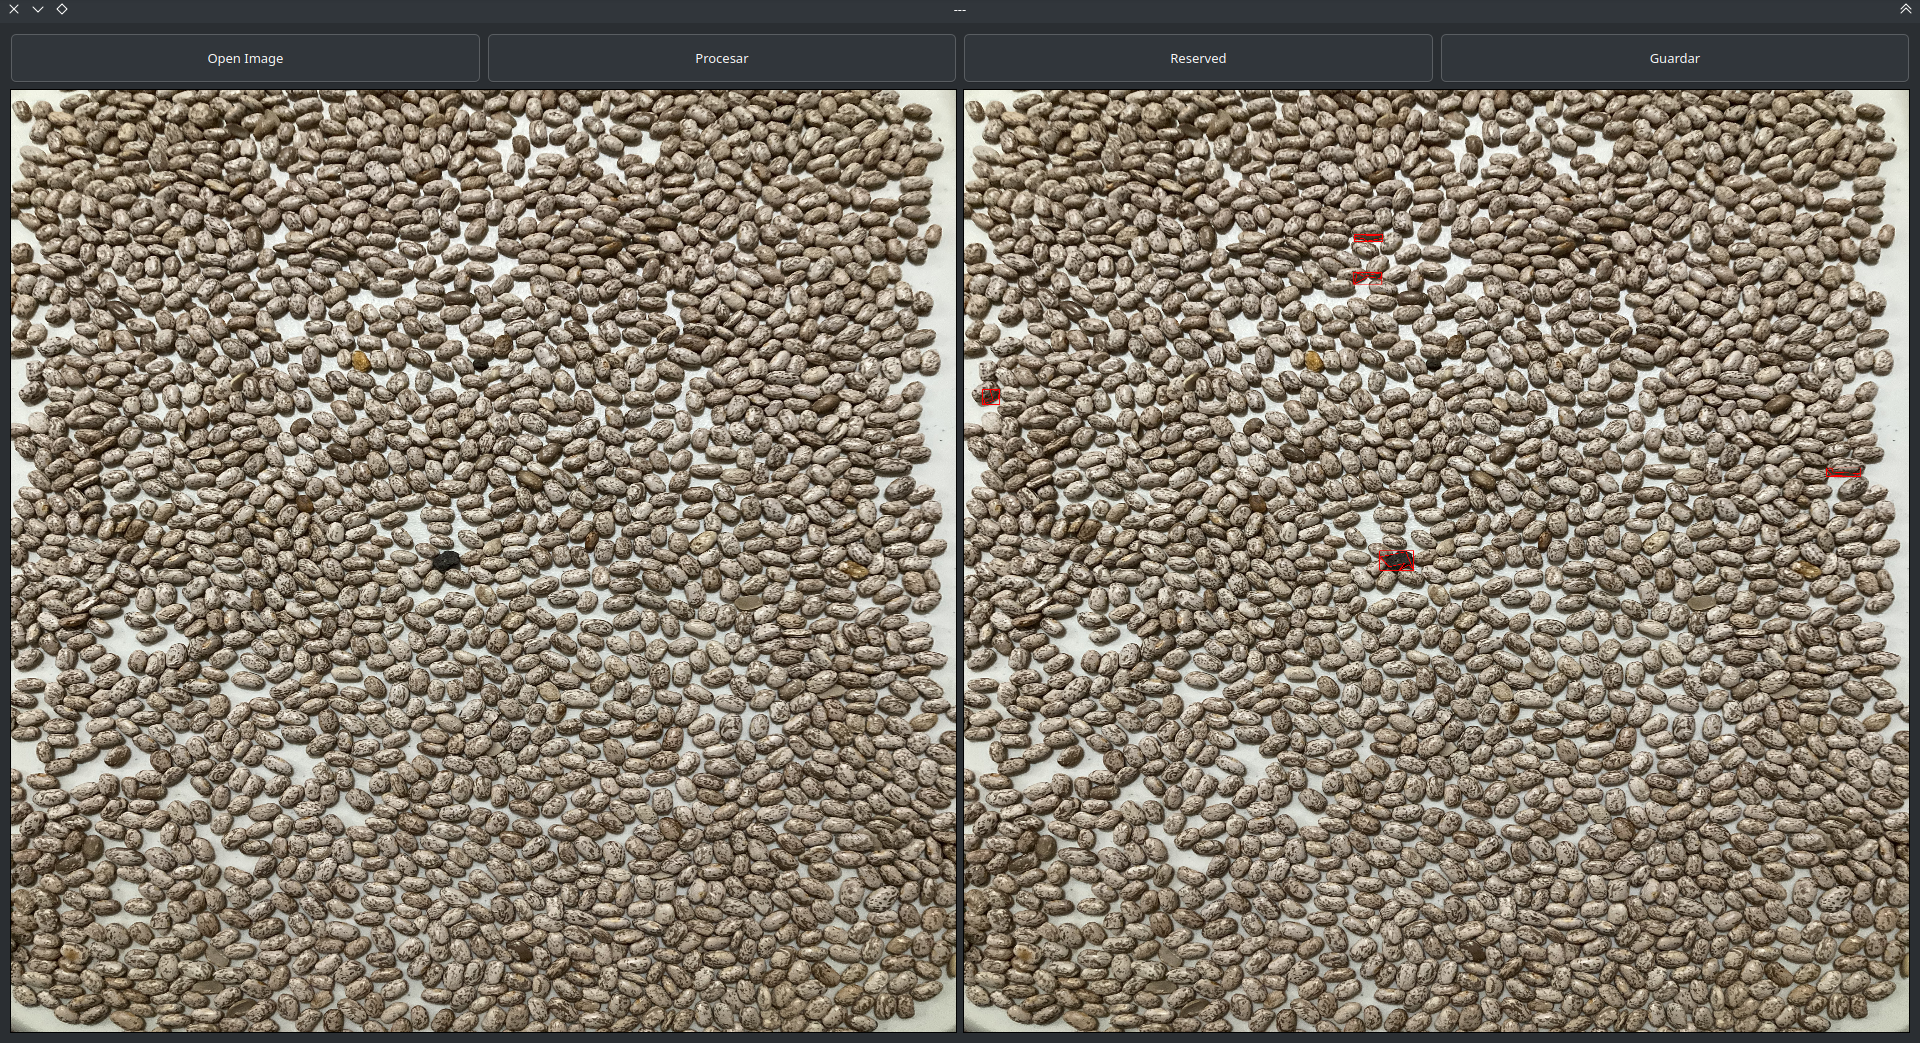
\includegraphics[width=\breite\linewidth]{images/test6.png}
            \caption{Resultados para test 6}
            \label{fig:test6}
        \end{figure}

        \begin{figure}[H]
            \centering
            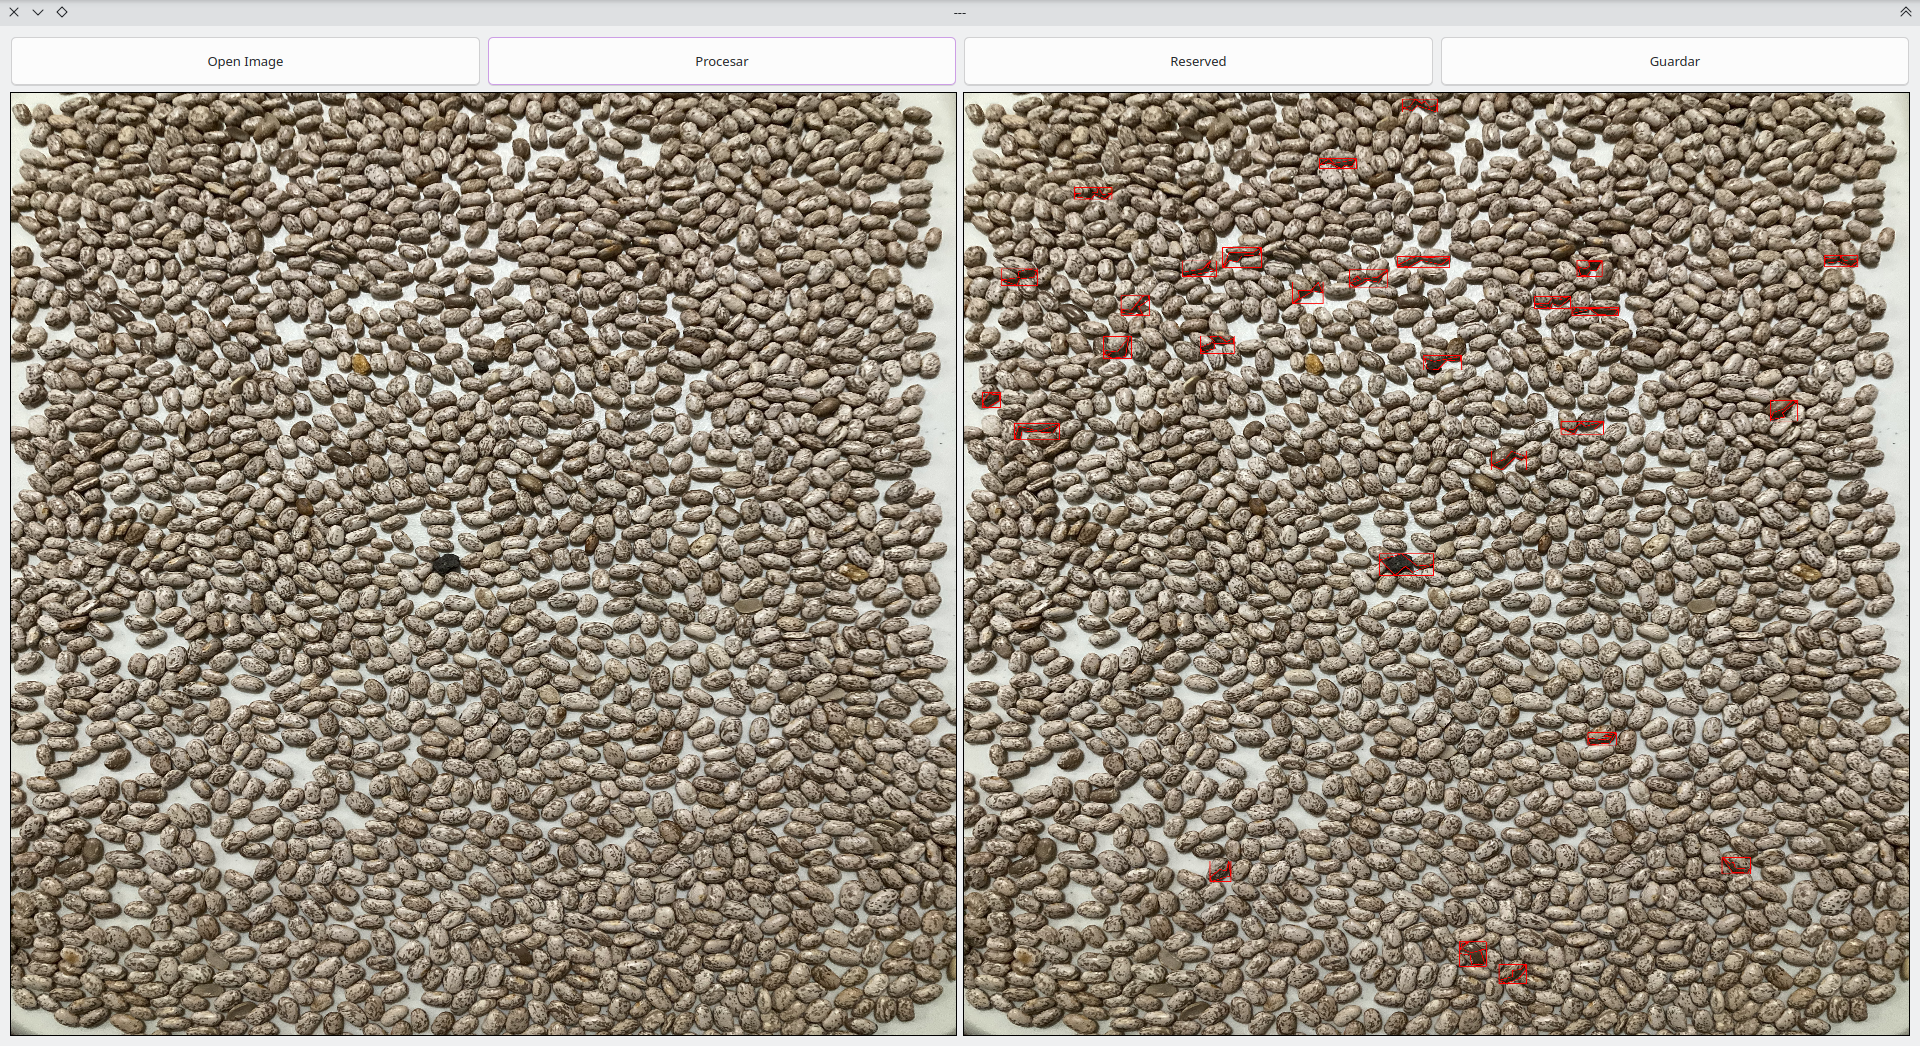
\includegraphics[width=\breite\linewidth]{images/test7.png}
            \caption{Resultados para test 7}
            \label{fig:test7}
        \end{figure}

        \begin{figure}[H]
            \centering
            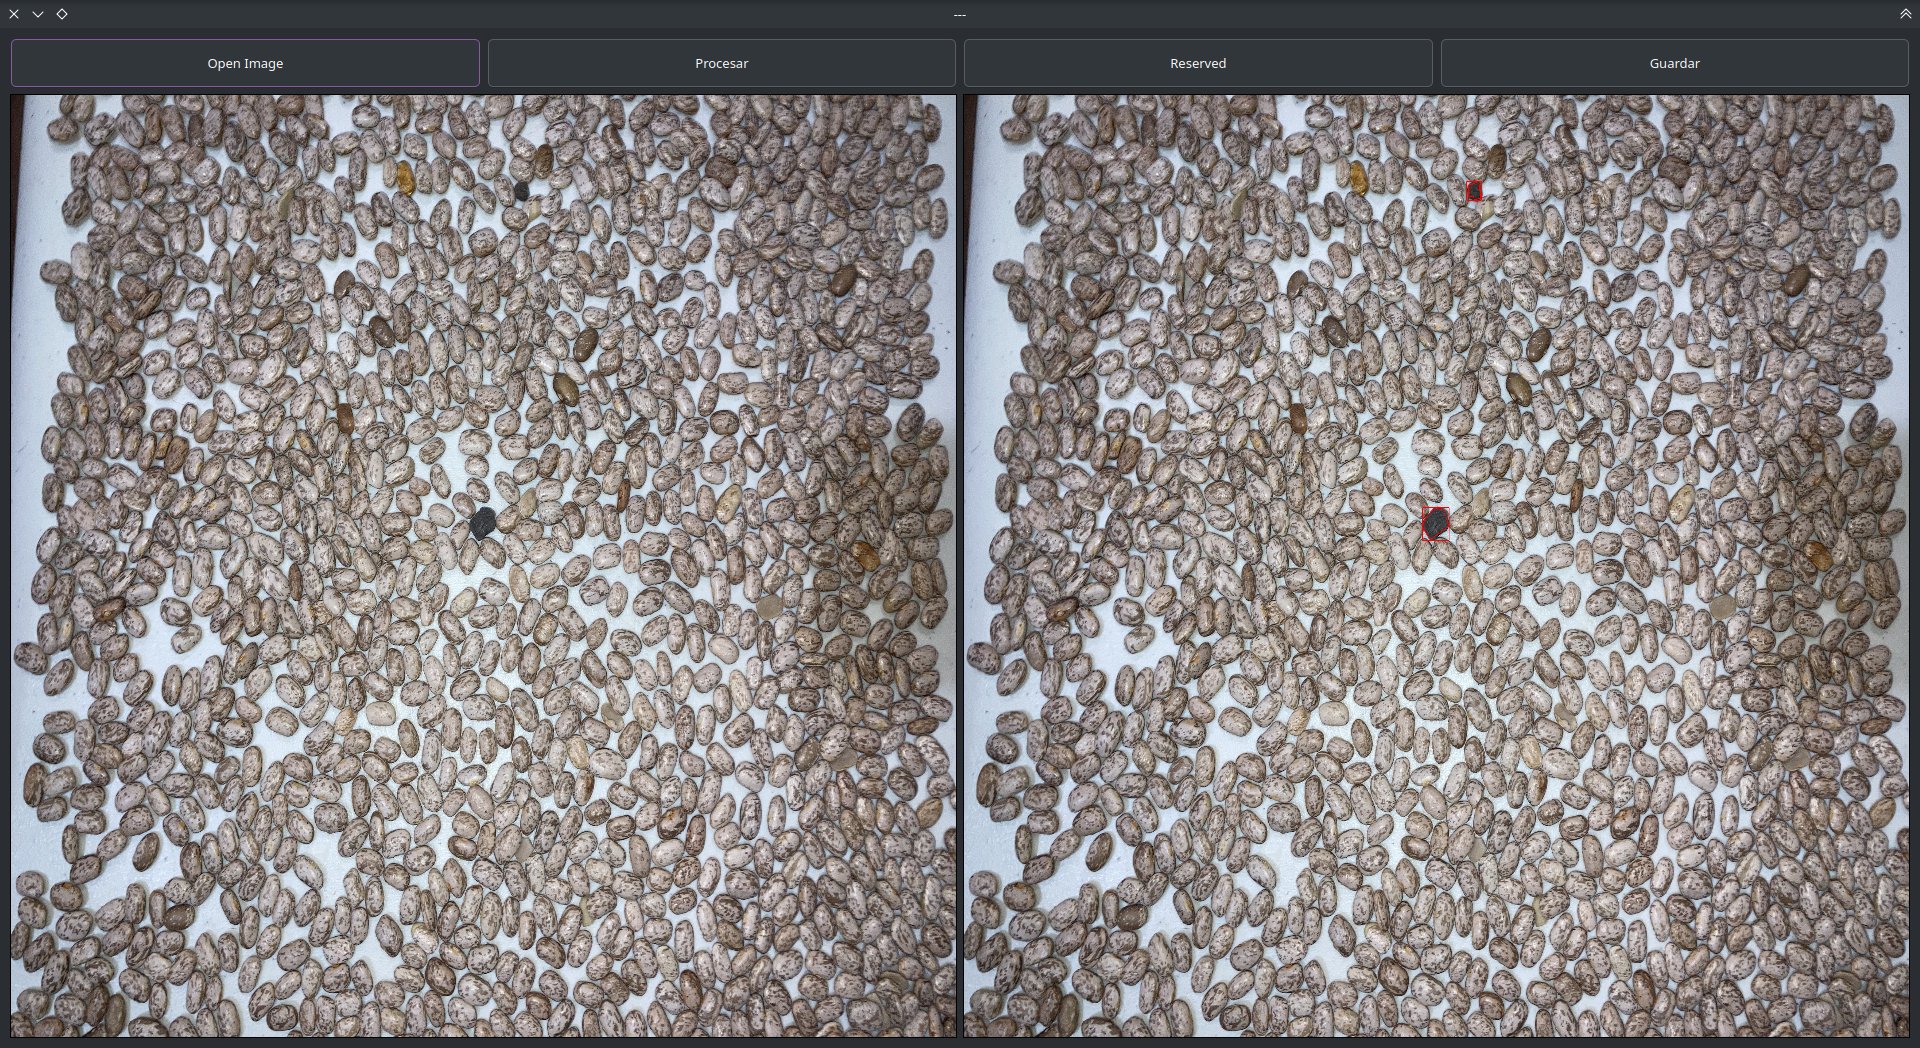
\includegraphics[width=\breite\linewidth]{images/test8.png}
            \caption{Resultados para test 8}
            \label{fig:test8}
        \end{figure}

        \begin{figure}[H]
            \centering
            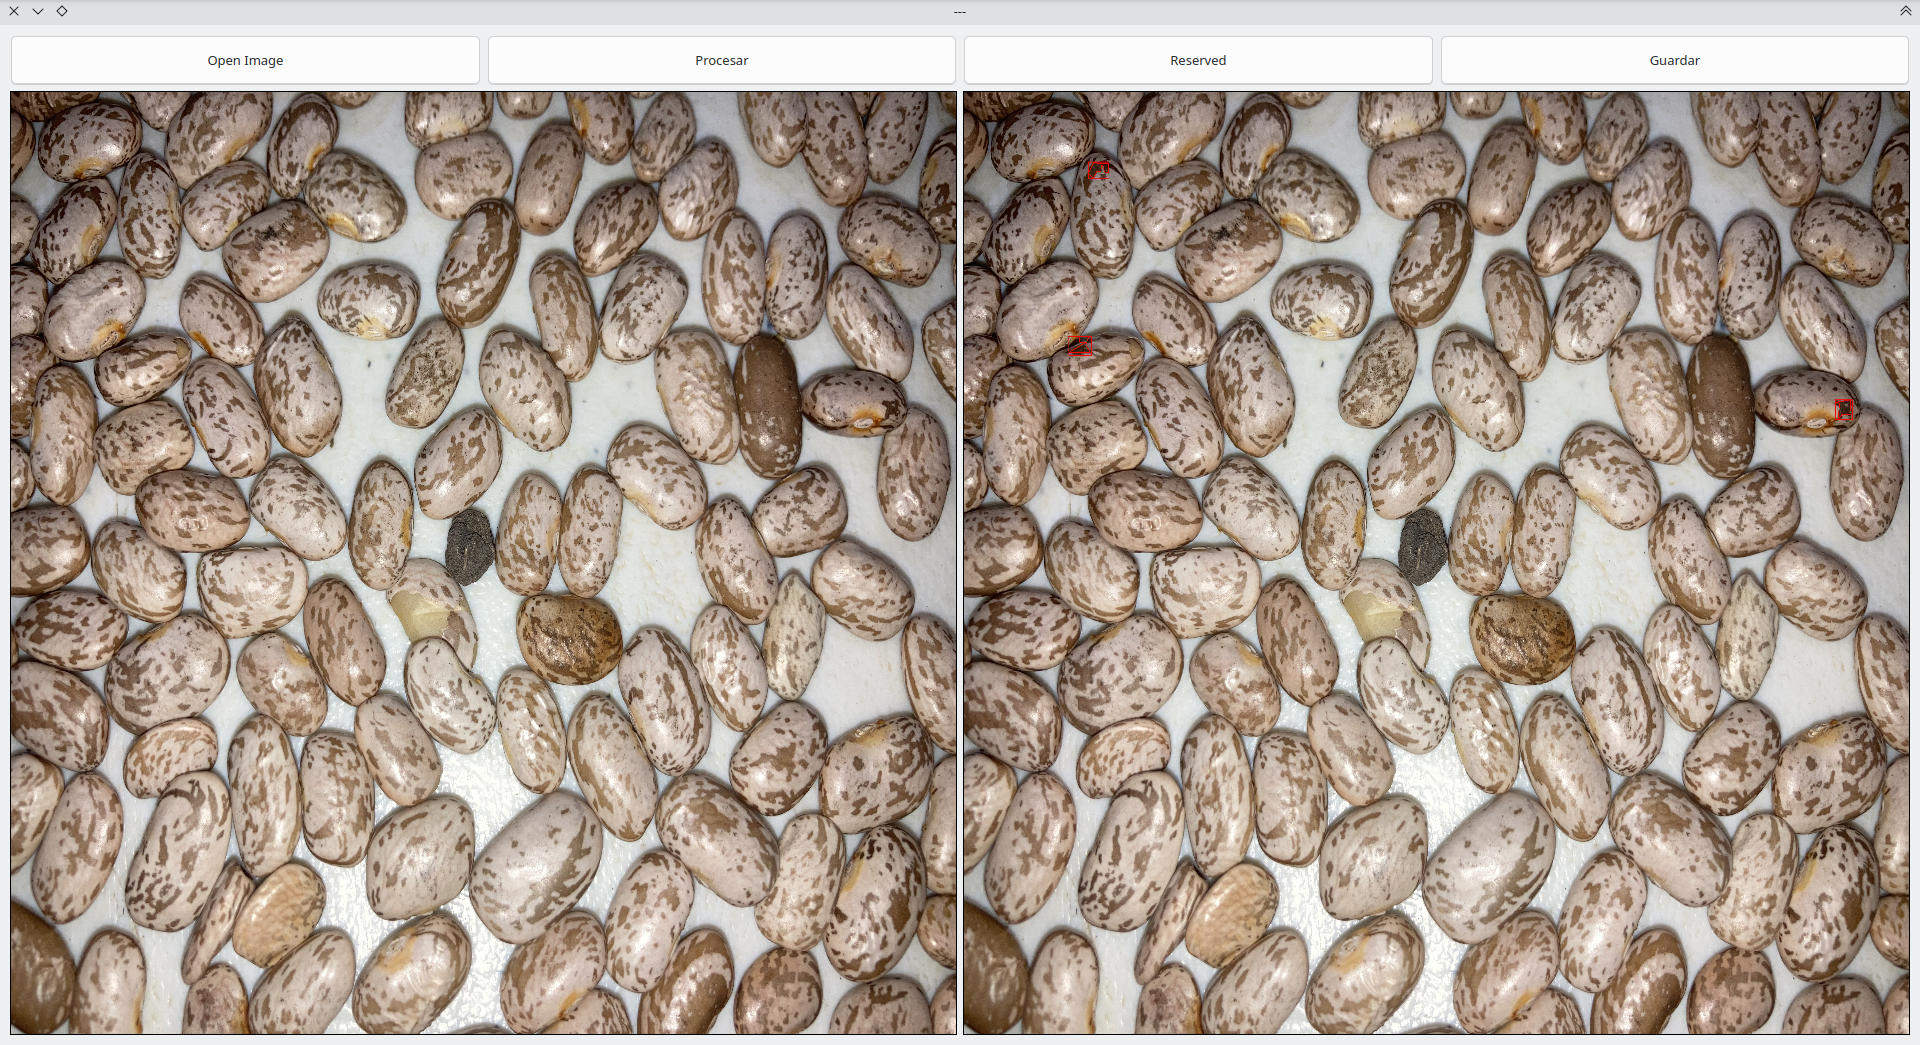
\includegraphics[width=\breite\linewidth]{images/test9.png}
            \caption{Resultados para test 9}
            \label{fig:test9}
        \end{figure}

        \begin{figure}[H]
            \centering
            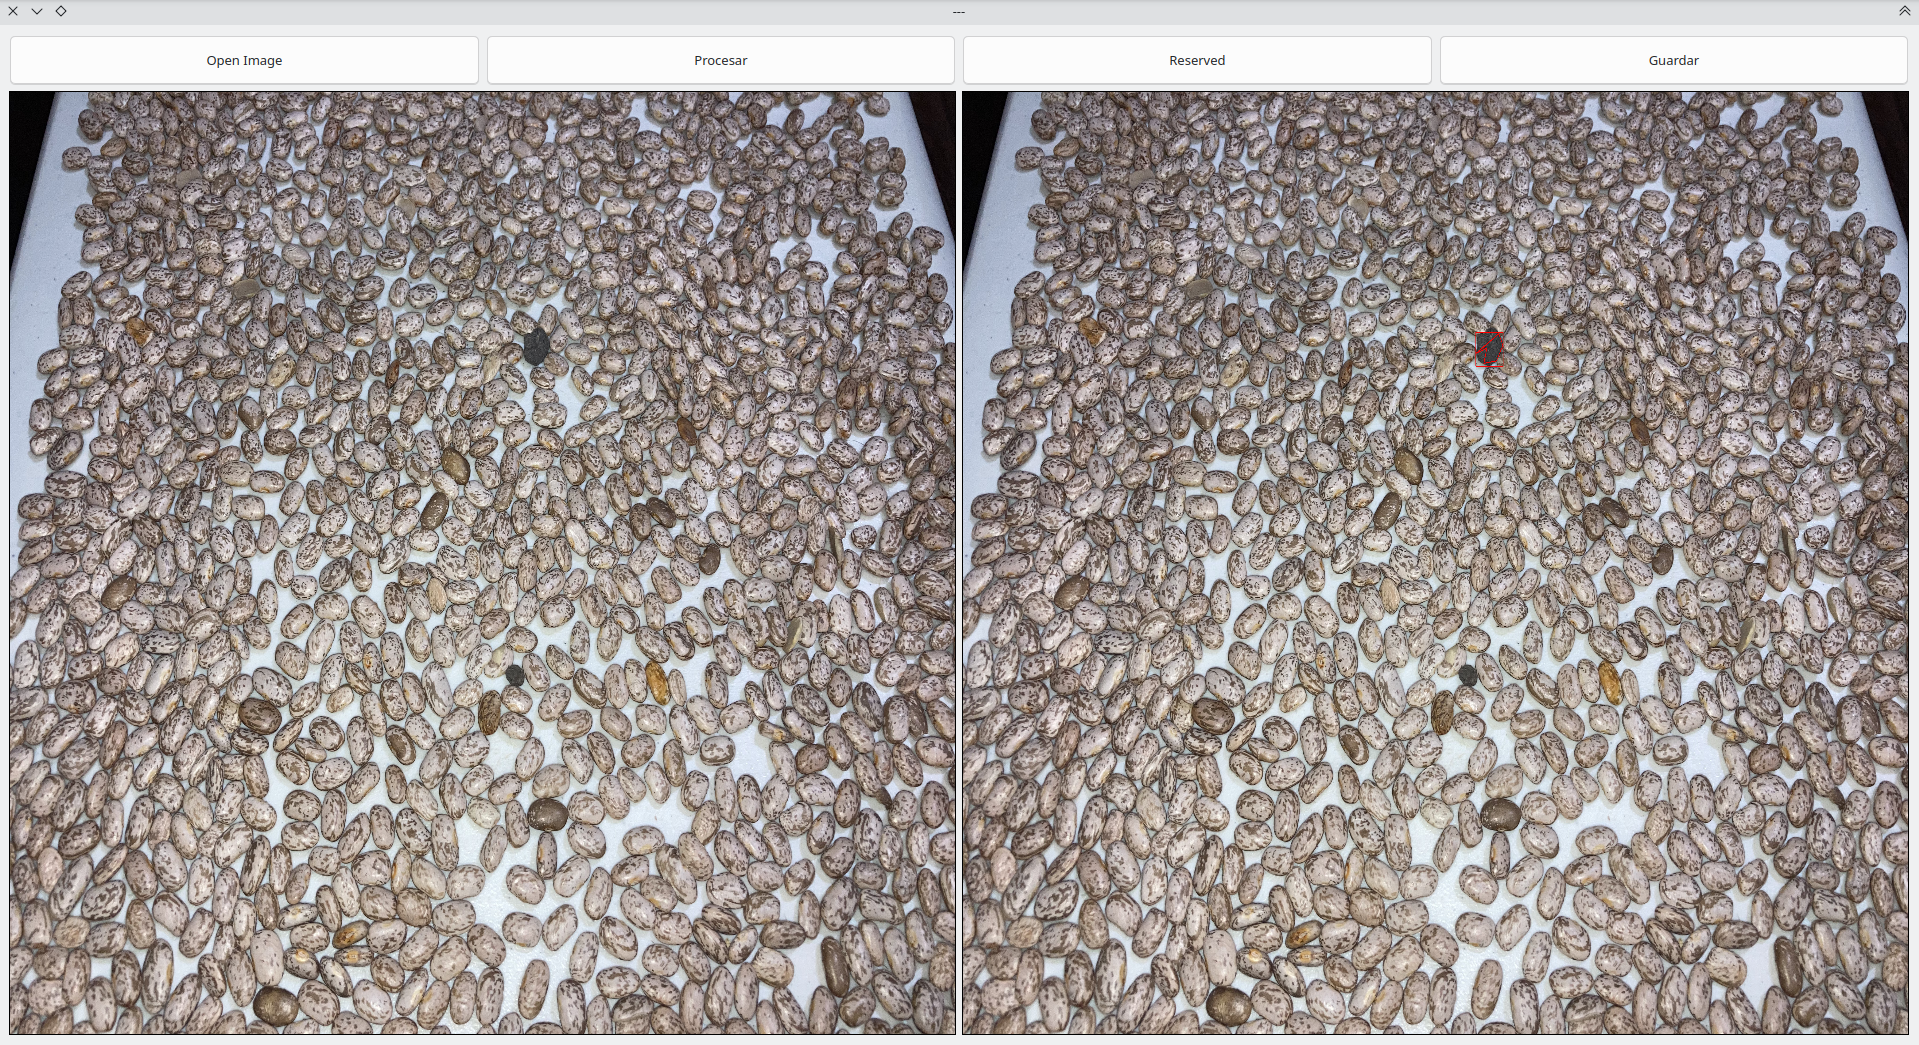
\includegraphics[width=\breite\linewidth]{images/test10.png}
            \caption{Resultados para test 10}
            \label{fig:test10}
        \end{figure}

    Como se puede observar en los test, principalmente el cambio que existe entre las imagenes es la forma en que se tomo la foto, al tener una forma distinta de procesamiento 

    % images/mascara_pintos.png
    \begin{figure}[H]
        \centering
        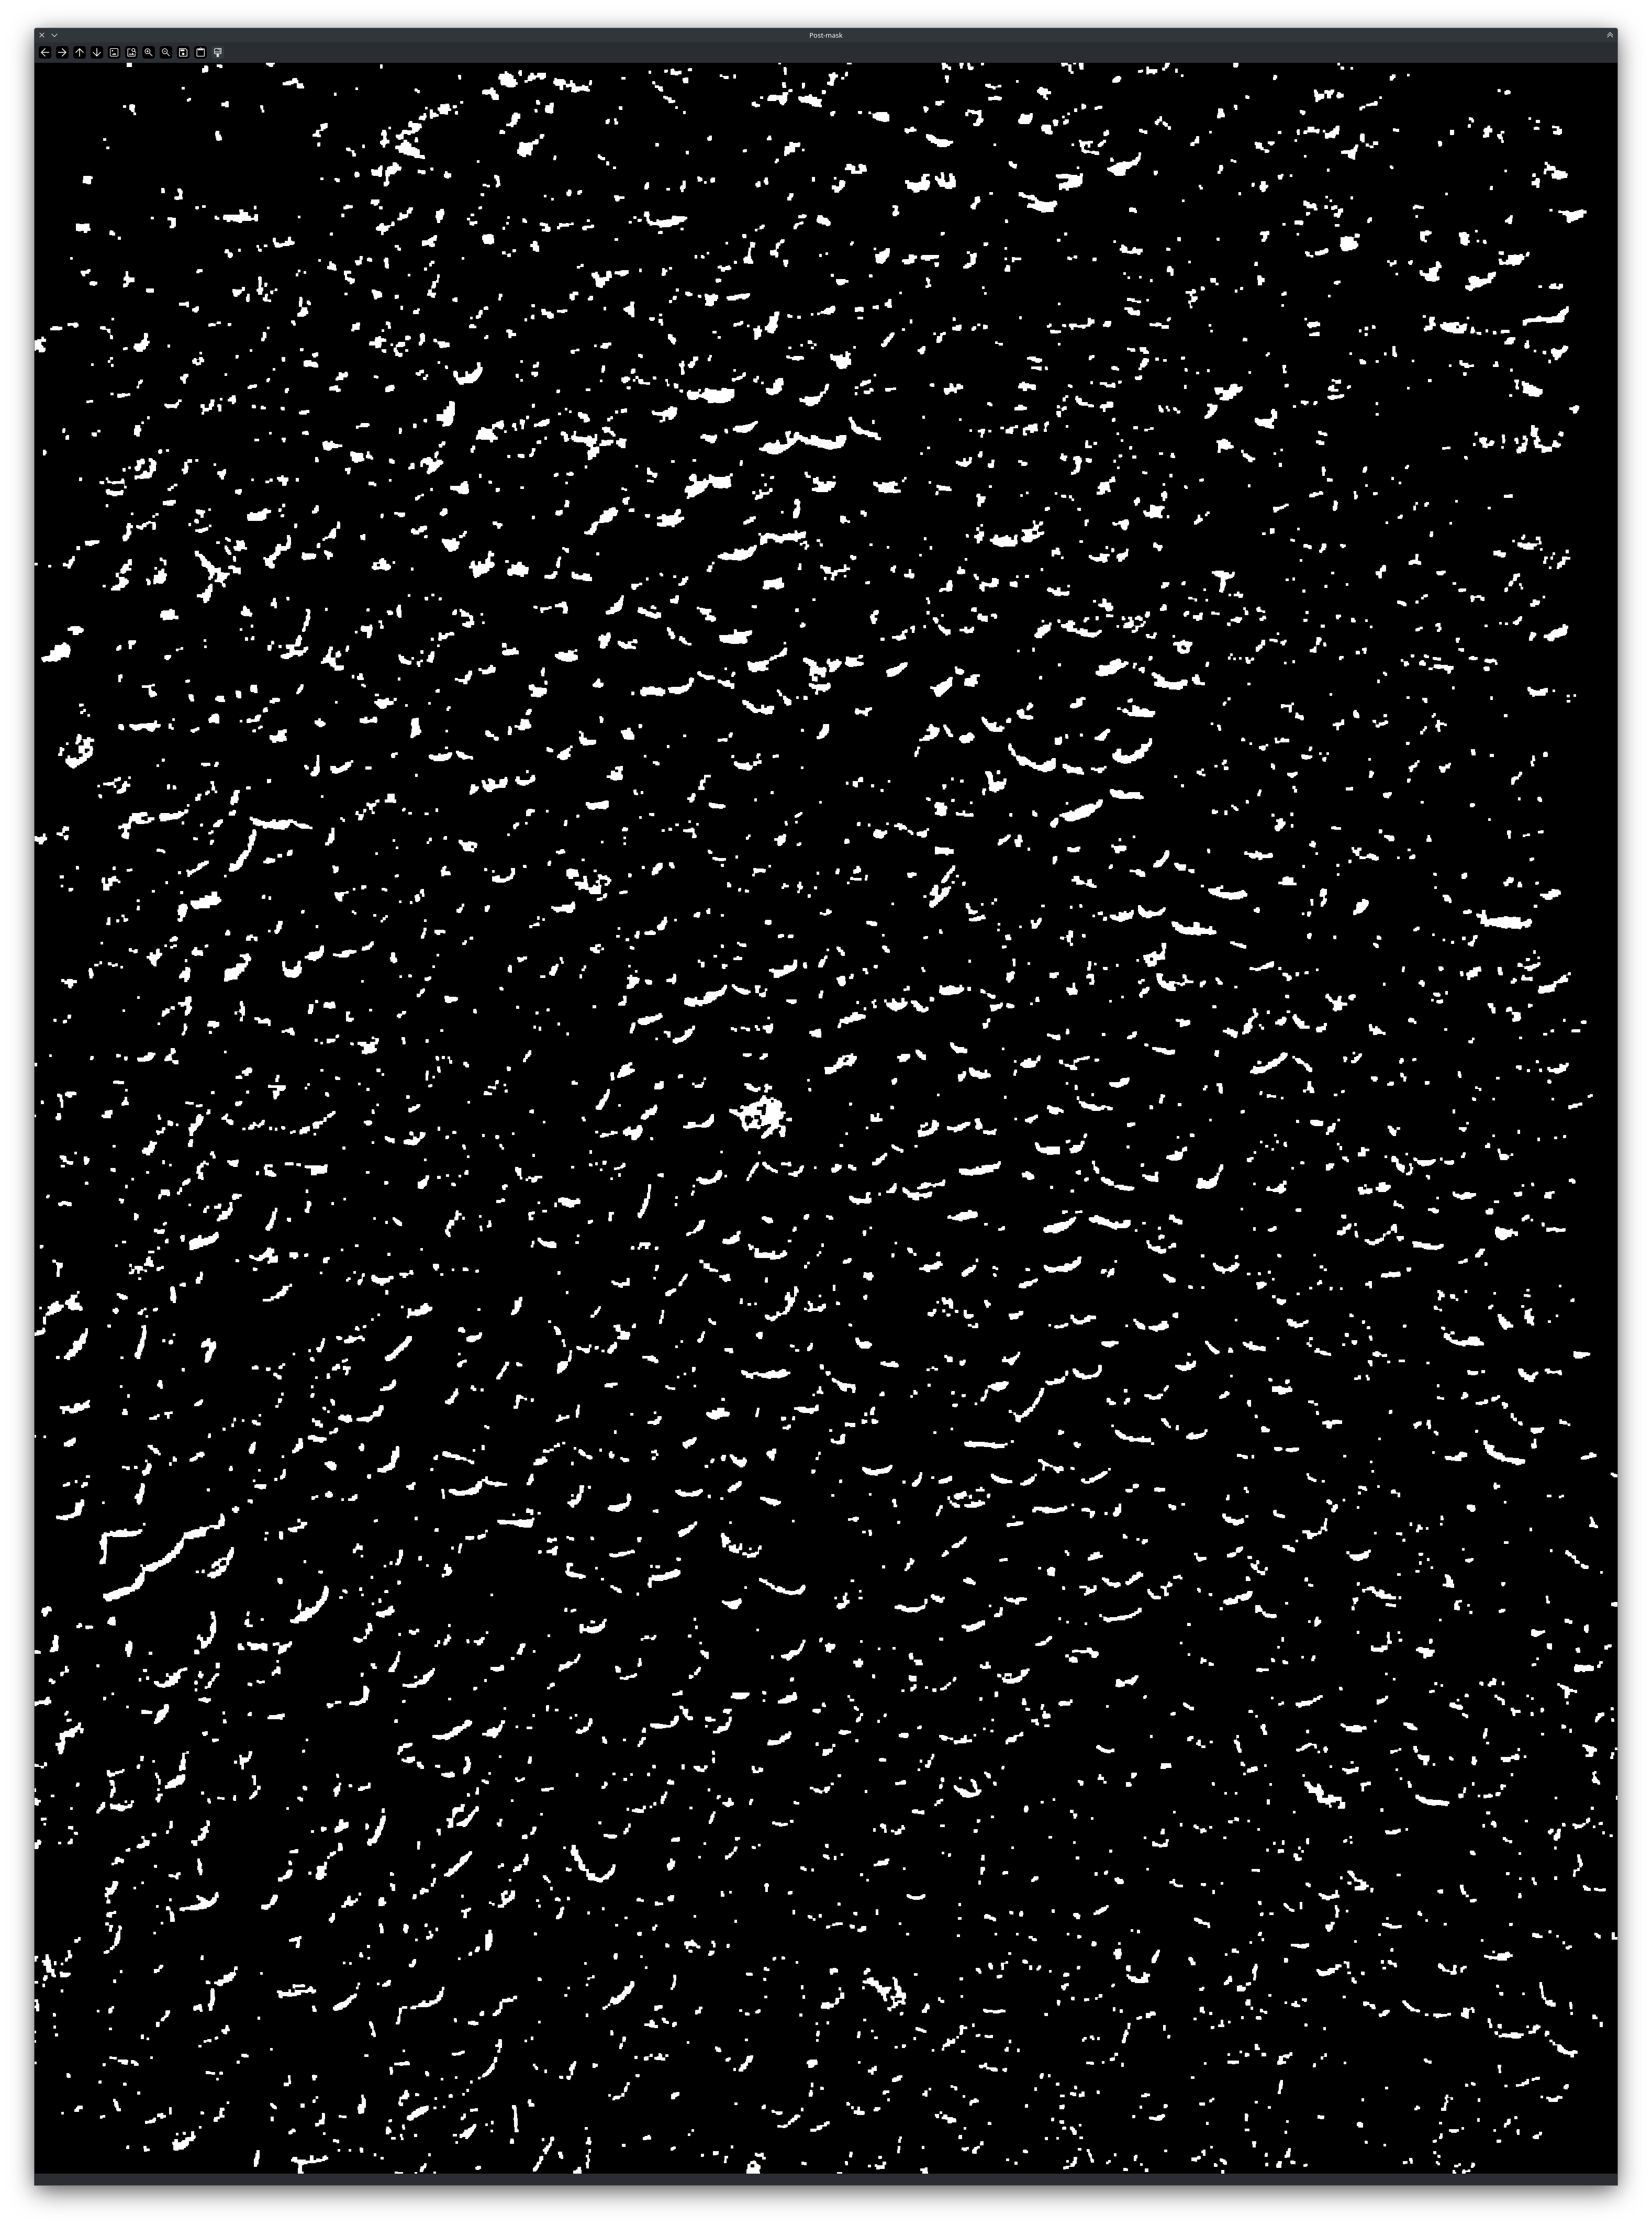
\includegraphics[width=\breite\linewidth]{images/mascara_pintos.png}
        \caption{Máscara de Piedras en Frijoles Pintos}
        \label{fig:mascara_pintos}
    \end{figure}

    % images/mascara_negros.png
    \begin{figure}[H]
        \centering
        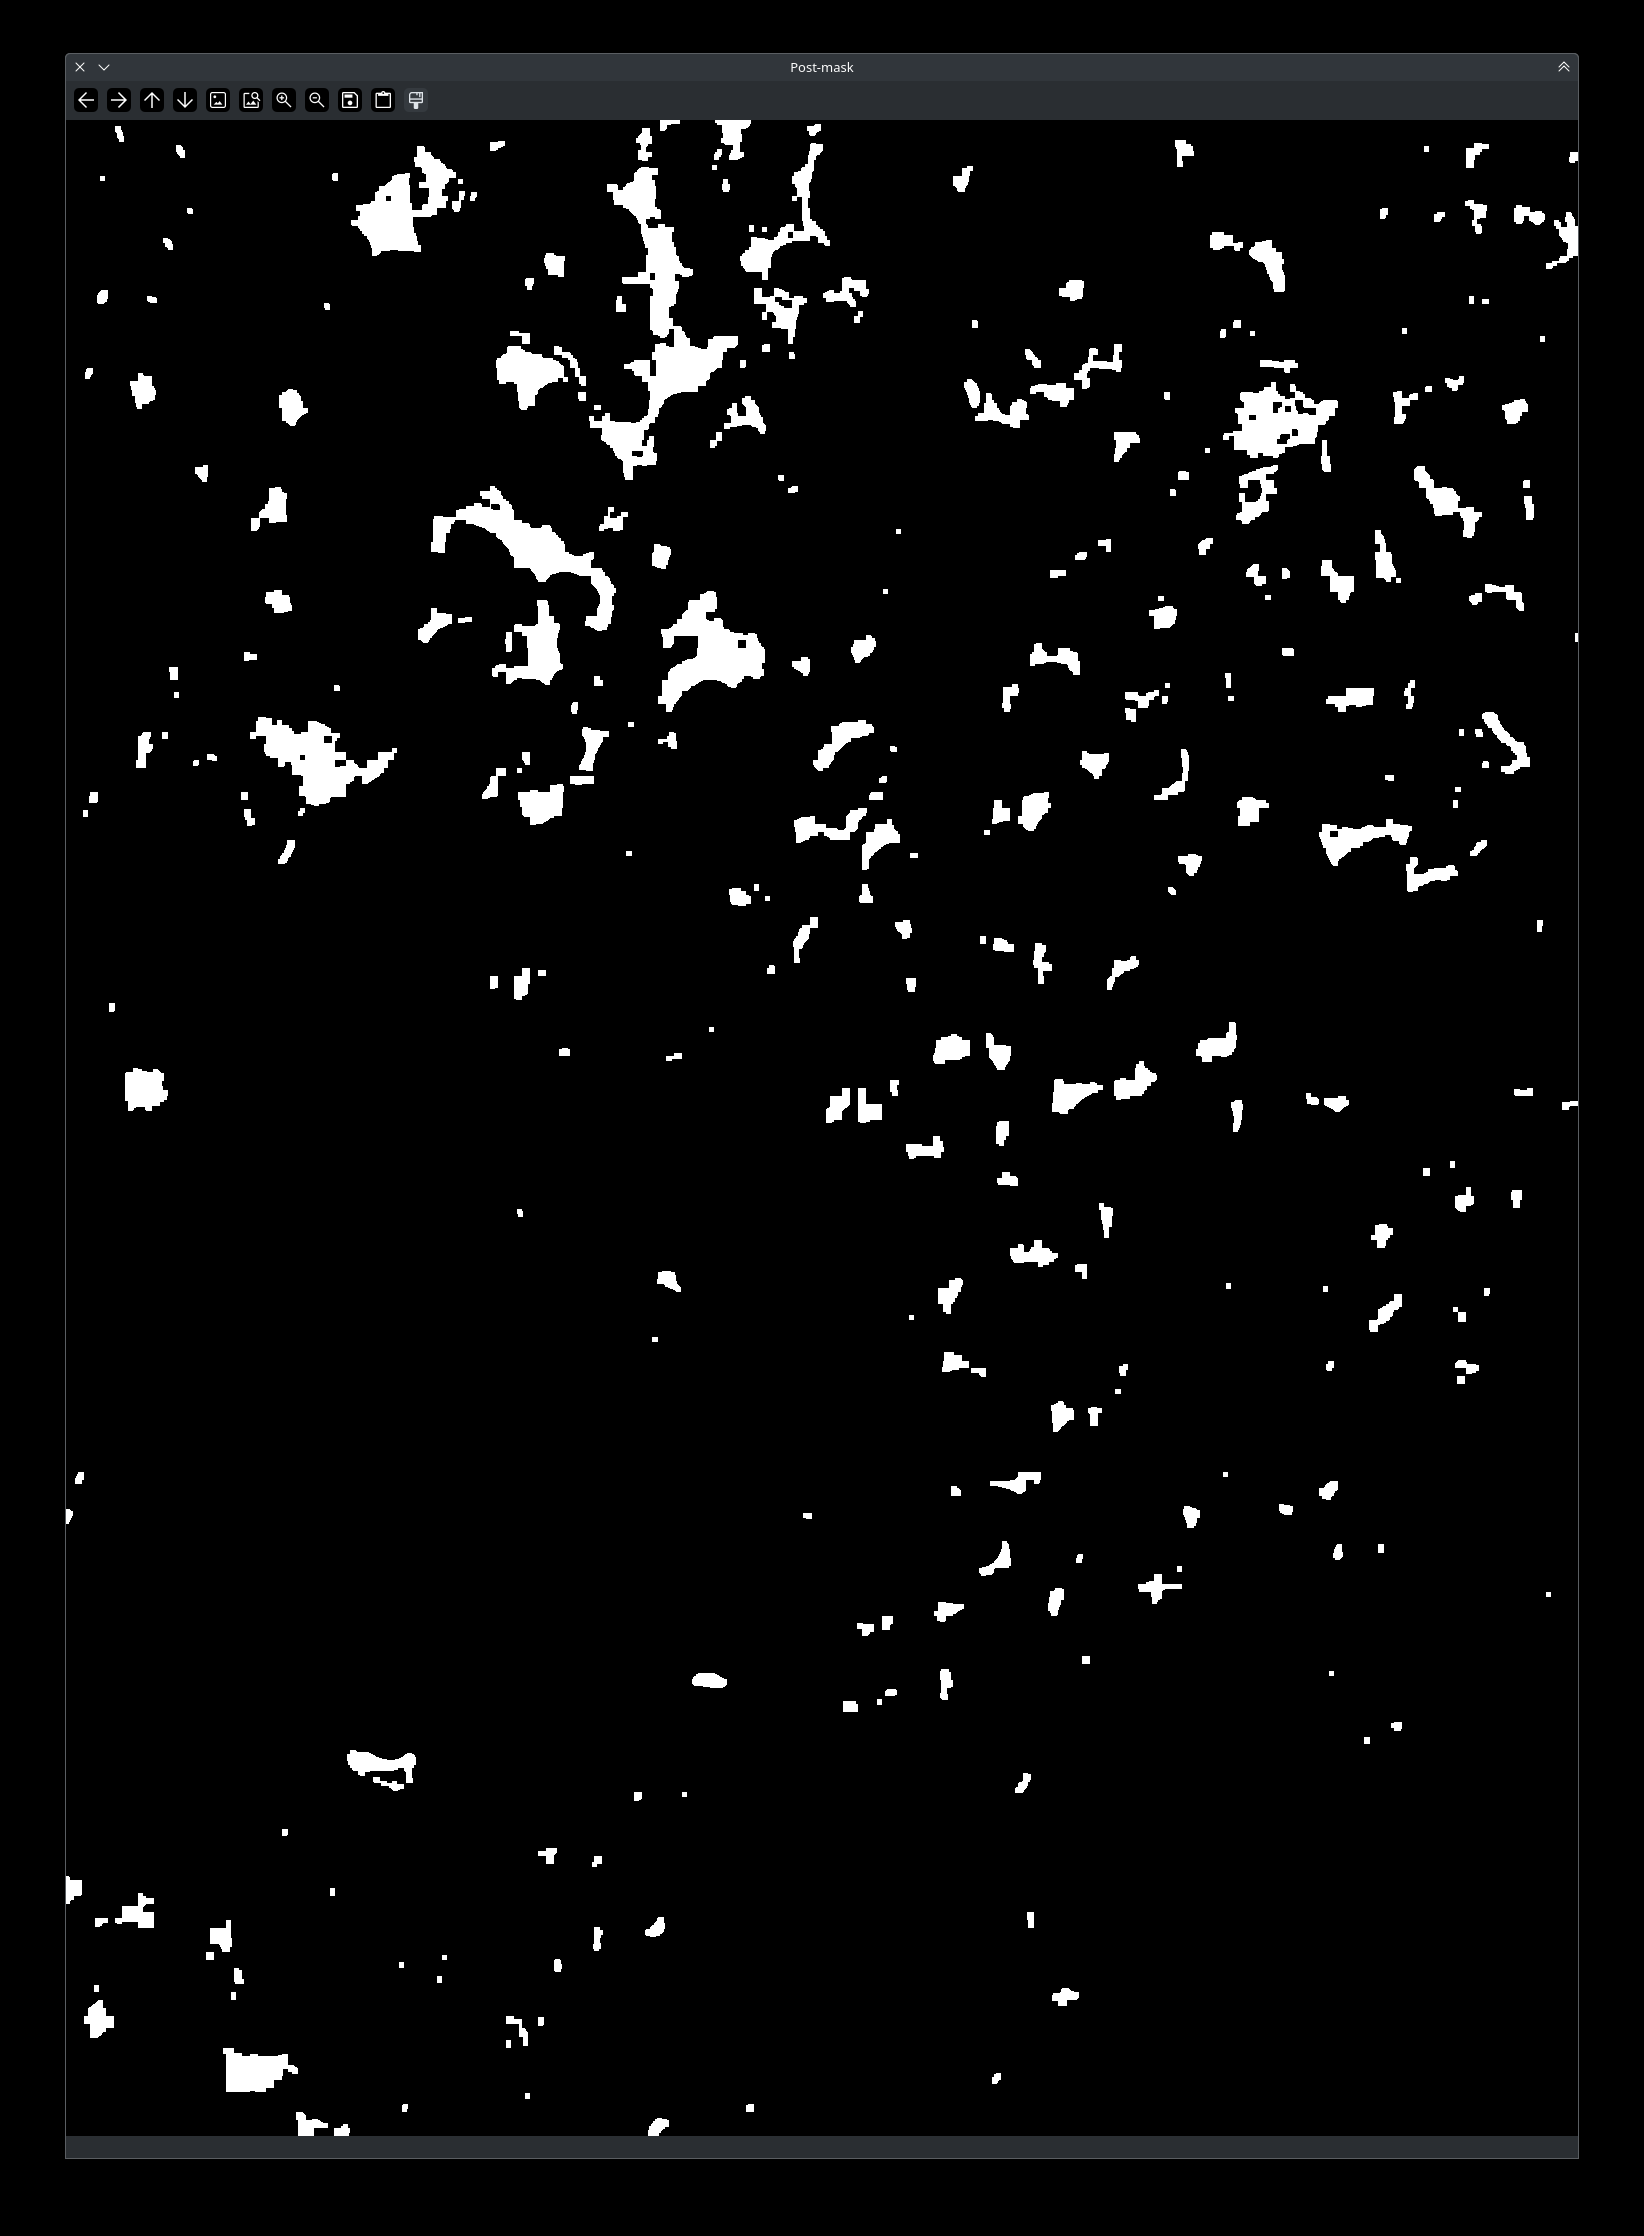
\includegraphics[width=\breite\linewidth]{images/mascara_negros.png}
        \caption{Máscara de Piedras en Frijoles Negros}
        \label{fig:mascara_negros}
    \end{figure}

%%%%%%%%%%%%%%%%%%%%%%%%%%%%%%%%%%%%%%%%%%%%%%%%%%%%%%%%%%%%%%%%%%%%%%%
\section{Conclusión}
    En este trabajo se propone un proyecto con la capacidad de detectar piedras entre un conjunto de frijoles usando solamente análisis de imágenes. Para lograr esto se usaron 2 características particulares de los frijoles; la diferente convexidad (para conocer la forma) que existe entre un frijol y una piedra, y las diferencias del color (esto haciendo uso de máscaras\cite{mask}). No se encontró algún proyecto en el cual podría inspirarse el nuestro 

    A pesar de la nula experticia en análisis de imágenes por parte del equipo, el resultado fue funcional, no obstante, simple; un sistema con cierta cantidad de asertividad, más no con una gran robustez debido a la inmensa variedad de piedras y frijoles existentes.
    

%%%%%%%%%%%%%%%%%%%%%%%%%%%%%%%%%%%%%%%%%%%%%%%%%%%%%%%%%%%%%%%%%%%%%%%
\nocite{*}
\addcontentsline{toc}{section}{Referencias} 
\printbibliography
%\balance

\end{document}